% shadow references (in comments) for thesis structure, approach, ..

\chapter{Introduction}


\section{Motivation}

With the large progress made since 2018 in NLP benchmarks by the last generation of artificial neural network language models, which are based on a  are based on a deep architecture of transformers layers and adopt a self-supervised learning approach, it has become increasingly important to understand what these model actually learn about human language \citep{hewitt2019structural, manning2020emergent, trotta2021monolingual}. \\
Investigating this serves multiple purposes, like providing insights for building better models, but it is also of interest for addressing research questions in linguistics \citep{hewitt2019structural}.  \\

(TODO: virgolettati da sintetizzare di seguito) \\

"Linguistic competence of neural language models (LMs) has emerged as one of the core sub-fields in NLP. "  (Cherniavskii et al. 2022 Acceptability Judgements via Examining the Topology of Attention Maps)
% "research paradigms" (Cherniavskii et al. 2022)

"more fine-grained evaluation tools may accelerate work on general-purpose neural network modules for sentence understanding. " \\
"studying the linguistic competence of ANNs bears on foundational questions in linguistics about the learnability of grammar."

(black boxes and explainability) : "the nature of the representations learned by these models is not properly understood." \citep{wilcox2018rnn}

"In addition to the insight these results provide about neural NLP systems, they also bear on questions central to cognitive science and linguistics, putting lower bounds on what syntactic knowledge can be acquired from string input alone"  \citep{hu2020systematic} 

% "We see two chief motivations that guide work on acceptability classification with ANNs by us and by others: First," 
% "Second, 
% better models: more performant, more efficient. Detect which linguistic phenomena they learn and which they don't.


% "Targeted syntactic evaluations have shown that these models [neural language models ] also implicitly capture many syntactic generalizations, ranging from subject–verb agreement to long-distance filler–gap dependencies (Linzen et al., 2016; Marvin and Linzen, 2018; Futrell et al., 2018; Wilcox et al., 2019b)" \citep{hu2020systematic}

%"similar developments in semantic evaluation (McCoy et al., 2019)" \citep{hu2020systematic}

% A particular interest of language in AI, is that it ..measures AI models with ..different concepts ..phenomena for which some of the standard ..alghoritmic/statistical or teory of information ..metrics, approaches, .. , don't work (eg. perplexity, ..probability estimation of next word, ..)

% transformer SotA :
% "transformer-based models, as they have become the benchmark for many NLP tasks in recent years (Vaswani et al., 2017; Devlin et al., 2019; Yang et al., 2019)"  \citep{lau2020furiously}. 
% transformers: much larger models, much more training data
% "Recent technological advances have led to an explosion of neural network-based LM architectures. The most popular ones are based on recurrent neural networks (RNNs) .. , LSTMs are still highly competitive (Melis et al., 2018)" \citep{marvin2018targeted}

% the above section should be renamed also "introduction"
% then have a more specific motitvation section on the motivation of this thesis within its line of research (targeted linguistic tests for language models)

% a  self-supervisedlearning approach. In self-supervised learning, a system is given no  explicit  labeling  of  raw  data,  but  it  is  able  to  construct  its own supervised learning problems by choosing to interpret someof  the  data  as  a  “label”  to  be  predicted \citep{manning2020emergent}

% The  canonical  casefor  human  language  is  the  language-modeling  task  of  trying to  predict  the  next  word  in  an  utterance  based  on  the  tempo-rally preceding words (Fig. 2). Variant tasks include the maskedlanguage-modeling  task  of  predicting  a  masked  word  in  a  text[a.k.a.  the  cloze  task  (11)]  and  predicting  the  words  likely  tooccur  around  a  given  word  (12,  13).  Autoencoders  (14)  canalso be thought of as self-supervised learning systems. Since noexplicit labeling of the data is required, self-supervised learningis  a  type  of  unsupervised  learning,  but  the  approach  of  self-generating supervised learning objectives differentiates it fromother unsupervised learning techniques such as clustering \citep{manning2020emergent}
% (that unsupervised models could not develop interesting knowledge of language) this  has  been  the  dominant  perspective  in  linguistics, where language models have long been seen as inadequateand having no scientific interest, even when their usefulness inpractical engineering applications is grudgingly accepted (15, 16). \citep{manning2020emergent}



% "A language model (LM) defines a probability distribution over sequences of words"  \citep{marvin2018targeted}



% "building better models": more performant and more data/computataion efficient
% The purpose of assessing which linguistic knowledge is acquired by language models based on neural networks: 
% - finding how/where/on what to improve the model, ..guiding research on further developing them for better performance, more data efficiency and computational efficiency
% - ..explainability, 
% - having a complementary measure of model performance, explaining performance (good or bad) in downstream application benchmarks, 
 
 
% BERT " implicitly learns to recover the rich latent structure of human language. "   (manning2020emergent)
 

% Addressing the question of how the linguistic knowledge of state-of-the-art language models (LMs) varies across linguistic phenomena \citep{warstadt2020blimp}

% "One promising line of research aims to crack open these ‘black boxes’ by investigating how" "language models perform on specially controlled sentences designed to draw out behavior that indicates representation of" "a syntactic dependency." \citep{wilcox2018rnn}



% "Many recent studies have searched for evidence that neural networks (NNs) learn representations ("\textit{linguistic knowledge}") that implicitly encode grammatical concepts. "  \citep{warstadt2020blimp}

% Purposes: to uncover linguistic phenomena where current state-of-the-art transformer-based language models lack human-like knowledge, to focus on investigating and improving those  \citep{warstadt2020blimp}.
% offer broad coverage of linguistic phenomena \citep{warstadt2020blimp} 

% indirect evidence about each model’s linguistic knowledge \citep{warstadt2020blimp}
% compare models in a fine-grained way \citep{warstadt2020blimp}.



\section{Research on linguistic tests on language models}
(TODO)
%(general introductory overview of previous studies, state of the art, chronicle history, ..)


\section{Island Effects and their assessment}

\subsection{Overview on island effects}

(TODO: sintetizzare i virgolettati di seguito) \\

"filler–gap dependencies are subject to numerous complex island constraints:  \citet{ross1968constraints} identified five syntactic positions in which gaps are illicit, dubbing them syntactic islands." \citep{wilcox2018rnn} \\
% "Even though the filler–gap dependency is flexible and potentially unbounded, it is not entirely unconstrained.

Examples: (..) \\

"open question whether these “island constraints” are true grammatical constraints, or whether they are effects of processing difficulty or discourse-structural factors (Ambridge and Goldberg, 2008; Hofmeister and Sag, 2010; Sprouse and Hornstein, 2014)" \citep{wilcox2018rnn} 

Argument from the poverty of the stimulus (APS):
"Because of their complexity and ubiquity, these dependencies have figured prominently in arguments that natural language would be unlearnable by children without a great deal of innate knowledge (Phillips, 2013) (cf. Pearl and Sprouse, 2013; Ellefson and Christiansen, 2000)" \citep{wilcox2018rnn} 

"The influential argument from the poverty of the stimulus (APS) ..  has been subject to much criticism (Pullum and Scholz, 2002)"  Geoffrey K. Pullum and Barbara C. Scholz. 2002. Empirical assessment of stimulus poverty arguments. The Linguistic Review, 18(1-2):9–50.

% psycholinguistic studies (Sprouse)

Wh-Island Constraint definition: 
"A gap cannot appear inside doubly nested clauses headed by wh-complementizers. This phenomenon is called the Wh-Island Constraint (WHC). "  \citep{wilcox2018rnn}

%Adjunct Island Constraint
%"We used three different prepositions to construct temporal adjuncts: ‘while’, ‘after’ and ‘before’." \citep{wilcox2018rnn}

\subsection{Island effects assessment in language models}

(TODO)

% Wilcox, Blimp, ..

\pagebreak

\section{Transformer-based language models}

% section on overview of NN language models, DL language models, transformers based language models

\subsection{Transformers and the Attention Mechanism}

Transformers  are "a neural network architecture,  without  any  recurrent  connections  (22),  which  takes  a sequence  of  words  (or  other  symbols)  as  input  and  produces a contextualized vector representation of each word as its out-put (Fig. 3). It contains many millions of trainable parameters in  a  number  of  layers,  typically  requiring  massive  amounts  of data  and  computation  to  train.  This  makes  Transformers  difficult  to  train,  but  also  highly  expressive  models  that  can  out-perform  other  contemporary  neural  networks  when  properly optimized" \citep{manning2020emergent}

"The key mechanism by which Transformers contextualize representations  is  multi-headed  attention  (see  Fig.  5)."  \citep{manning2020emergent} 
"attention is a kind of \textbf{generalized dot product}" % (Manning Lecture) https://www.youtube.com/watch?v=aKO1Yok6e4Q&list=PLGJm1x3XQeK0gmqfRkP-VmrEf4UYx5IDW&index=4
which models all pairwise interactions between words.

"Attention(23) dynamically assigns a weight to every pair of words in the sequence, indicating how much the model should “pay attention to” the first word when computing the representation of the second one."  \citep{manning2020emergent}
"Transformers use multiple attention heads in parallel, where  each  head  can  potentially  capture  a  completely  different word–word relation. Transformers aggregate the information from each head to produce a single output vector representation for each word in the sequence." \citep{manning2020emergent}
% "We provide more mathematical detail below" \citep{manning2020emergent}

\begin{figure}[H]
	\centering
	\includegraphics[width=1\textwidth]{images/Chapter1/attention-manning-pnas.png} 
	\caption{Overview of the attention mechanism, taken from \citet{manning2020emergent} (TODO: request permission, pnas licence is CC ND)} 
	\label{fig:manning_attention} 
	\medskip
	\small
	..
\end{figure}

% a non-recurrent architecture, called the Transformer \citep{vaswani2017attention} 
The lack of recurrence in the transformers architecture "enables greater within-training-example parallelization, at the cost of quadratic complexity in the input sequence length" \citep{liu2018generating} 

% Jurasfy book (draft new 3rd edition), ch.10 .. \citep[ch.9-10]{jurafsky2021speech} 

the terminology used to describe the Transformer: "the attention is a function of a query (Q) and set of key (K) and value (V ) pairs" \citep{liu2018generating} 
% multi-head self-attention of the Transformer

% to reduce memory usage, limiting the dot products between Q and K

% "projecting the tokens into the query, key, and value embeddings"

% decoder-only vs encoder-decoder
% what is an attention head? See "explorable transformers" 

% explorable Bert (online javascript demo): \href{https://huggingface.co/exbert/?model=gpt2&modelKind=bidirectional&sentence=The%20girl%20ran%20to%20a%20local%20pub%20to%20escape%20the%20din%20of%20her%20city.&layer=0&heads=..0,1,2,3,4,5,6,7,8,9,10,11&threshold=0.7&tokenInd=null&tokenSide=null&maskInds=..&hideClsSep=true}{exbert}

% possible TODOs: 
% -give detailed description of each layer dimensions (eg vocab x ..) 
% -compare bert and gpt architecture
% -explain output of gpt and bert

% save the checkpoints of gpt and bert with pythorch inspect the layers

% is dot product in attention a form of linear basis expansion?
% (from machine learning course lectures: name of "augmenting" the input ..)(..appropriate name for semantic info addition?)(LBE, linear basis expansion)(..equivalent to semantic augmentation of the input?)

% schema of the self-attention mechanism (multipling on prev inputs)

% (horizontal vs vertical attention?)

% criticism of attention mechanism (refs)
% alternative attention mechanism
% attention mechanism more efficient for NLP
% auto pruning of attention heads?


Training objective function, cross-entropy loss:
 "During training, the probability assigned to the correct word is used to calculate the cross-entropy loss for each item in the sequence. As with RNNs, the loss for a training sequence is the average cross-entropy loss over the entire sequence." (Jurasfky 3rd ed. ch.9)(figure 9.21)

% query, key, value

transformer blocks "Each provides a multi-headed self-attention unit over all input words, allowing it to capture multiple dependencies between words, while avoiding the need for recurrence. With no need to process a sentence in sequence, the model parallelizes more efficiently, and scales in a way that RNNs cannot" \citep{lau2020furiously}


\subsection{Traditional unidirectional language models (Gpt2)}

% Traditional LM can "produce sentence probabilities (density estimation) " \citep{salazar2020masked}

% todo: definition of token, distinction from words
% todo: definition/mention of tokenizations, and subword units

Conventional language models, like LSTM, TDLM, and GPT2, are unidirectional, they predict the probability of a token using only past tokens
% "conventional language models (LMs) predict wt using only past tokens W<t := (w1; : : : ; wt-1)." 
"the input [to GPT2] is a sequence of previously seen words, which are then mapped to embeddings (along with their positions) and fed to multiple layers of ‘‘transformer blocks’’ before the target word is predicted" ""Much of its power resides in these transformer blocks" \citep{lau2020furiously}


The unidirectionality of conventional LMs allows to estimate log probabilities for a sentence W via the chain rule \citep{salazar2020masked} \\
$log P_{LM}(W) = \sum_{t=1}^{|W|} log P_{LM}(w_t | W_{<t}$" 
% "which can be used out of the box to rescore hypotheses in end-to-end speech recognition and machine translation (Chan et al., 2016; Gulcehre et al., 2015), and to evaluate sentences for linguistic acceptability (Lau et al., 2017)."  \citep{salazar2020masked}

"Given a unidirectional language model, we can infer the probability of a sentence by multiplying the estimated probabilities of each token using
previously seen (left) words as context (Bengio et al., 2003):" \citep{lau2020furiously}
% →P (s) = |s| Y i =0 P(wi|w<i)
% "where s is the sentence, and wi a token in s. LSTM, TDLM, and GPT2 are unidirectional models, so they all compute sentence probability as described" \citep{lau2020furiously}

% The GPT architecture \citep{radford2018improving} ..
% TODO: intended meaning of the loss measure, sentence likelihood, contrast with sentence acceptability, .., ungrammatical sentences that are more likely than rarer grammatical ones, ..)
% (math formulas of Gpt output, activation functions..)


% C’è da aggiungere che la loss del modello gpt (score PenLP), usato come misura di accettabilità, è in realtà una stima globale della ..likelihood della frase (reference for this .. from gpt paper or other paper on ..transformers based language models). Ciò non corrisponde esattamente ad un giudizio di accettabilità/grammaticalità. Infatti, potrebbe darsi il caso, che una frase piuttosto comune (..) ma con un errore (sintattico, semantico, o altro) riceva una ..loss/likelihood maggiore di una frase. grammaticalmente corretta ma “rara”, o meglio, che usa un costrutto ricercato.. (es. ..).

% recap: average cross entropy loss should be how the gpt2 output loss is calculated (add img with Jurafsky figures)
% ..check with transformers code how it's actually calculated
% (calls torch CrossEntropyLoss, which "computes the cross entropy loss between input and target")

% gpt forward method:

% https://www.overleaf.com/learn/latex/Code_listing
%\begin{lstlisting}[language=Python]
%
%# modeling_gpt2.py
%
%class GPT2Model(GPT2PreTrainedModel):
%    def __init__(self, config):
%    	..
%    def forward(
%	    self,
%	    input_ids=None,	
%	    ..
%	 ):
%	 	..
%	 	return BaseModelOutputWithPastAndCrossAttentions(
%		 	last_hidden_state=hidden_states,
%		 	past_key_values=presents,
%		 	hidden_states=all_hidden_states,
%		 	attentions=all_self_attentions,
%		 	cross_attentions=all_cross_attentions,
%	 	)
%
%class GPT2LMHeadModel(GPT2PreTrainedModel):	
%
%	def __init__(self, config):
%		self.transformer = GPT2Model(config)
%		self.lm_head = nn.Linear(
%			config.n_embd, 
%			config.vocab_size, bias=False
%		)
%	
%	def forward(input_ids=None, ..	labels=None, ..):
%		r"""labels (`torch.LongTensor` of shape 
%		`(batch_size, sequence_length)`, *optional*):
%		Labels for language modeling. Note that the labels **are shifted** inside the model, i.e. you can set
%		`labels = input_ids` Indices are selected in 
%		`[-100, 0, ..., config.vocab_size]` 
%		All labels set to `-100` are ignored (masked), the loss is only computed for labels in `[0, ..., config.vocab_size]`
%		"""
%		
%		transformer_outputs = self.transformer(input_ids, ..)
%		hidden_states = transformer_outputs[0]  # last_hidden_state or hidden_states?
%		lm_logits = self.lm_head(hidden_states)
%		shift_logits = lm_logits[..., :-1, :].contiguous()
%		shift_labels = labels[..., 1:].contiguous()
%		
%		loss_fct = CrossEntropyLoss()
%		loss = loss_fct(
%			shift_logits.view(-1, shift_logits.size(-1)), 
%			shift_labels.view(-1)
%		)
%	
%		return CausalLMOutputWithCrossAttentions(
%			loss=loss,
%			..
%		)
%\end{lstlisting}

% todo, clarify: cross entropy fun takes (input, target), but gpt2 calls it with (logits, labels), which are both the sentence_ids (the ids of the tokens in the sentence)

% pytorch CrossEntropyLoss formula:

%\begin{lstlisting}
%	
%class CrossEntropyLoss(_WeightedLoss):
%	def forward(self, input: Tensor, target: Tensor) -> Tensor:
%		return F.cross_entropy(input, target, ..)
%		
%		lm_logits = self.lm_head(hidden_states)
%\end{lstlisting}
%
%usage:
%\begin{lstlisting}
%model_output = model(
%sentence_ids_in_batch_as_tensor,
%labels=sentence_ids_in_batch_as_tensor,
%)
%loss = model_output.loss
%\end{lstlisting}

%From the pytorch cross entropy documentation, about the two parameters input and labels:
%
%"The input is expected to contain raw, unnormalized scores for each class. input has to be a Tensor of size (C)(C) for unbatched input, (minibatch, C)(minibatch,C) "

..

\subsection{Bidirectional language models (BERT)}


"BERT (Devlin et al., 2019) and its improvements to natural language understanding have spurred a rapid succession of contextual language representations (Yang et al., 2019; Liu et al., 2019; inter alia) which use larger datasets and more involved training schemes. Their success is attributed to their use of bidirectional context, often via their masked language model (MLM) objectives." \citet{salazar2020masked}

"The self-supervision task used to train BERT is the masked language-modeling  or  cloze  task,  where  one  is  given  a  text  in which  some  of  the  original  words  have  been  replaced  with  a special  mask  symbol.  The  goal  is  to  predict,  for  each  masked position,  the  original  word  that  appeared  in  the  text  (Fig.  3).To perform well on this task, the model needs to leverage the surrounding context to infer what that word could be." \citep{manning2020emergent}


% "MLMs model all pairwise interactions $w_s$ and $w_{s'}$ via dot product attention" "conditioned on past and future context" \citep{salazar2020masked}
% PLLs of models like EMLO would have different properties from [BERT] (e.g., their cross-entropies in Figure 4 may be convex instead of flat)  \citep{salazar2020masked}

% On the use of the Softmax, the logistic function (or possibly a probability measure based on the logistic function, but dividing all values for the total sum)


"BERT’s MLM objective can be viewed as stochastic maximum pseudolikelihood estimation (MPLE) \citet{wang2019bert}(Besag, 1975) on a training set  .. " \citep{salazar2020masked}
"In this way, MLMs learn an underlying joint distribution whose conditional distributions 
$w_t | W_{\setminus t}$ 
are modeled by masking at position $t$."  \citep{salazar2020masked}
% We include a further discussion in Appendix B" \citep{salazar2020masked}



% \pagebreak



\chapter{Related work}

The previous works closest to ours are those by \citet{wilcox2018rnn, hu2020systematic, sprouse2016experimental}, which use a factorial test design and test on island effects, on neural language models for \citet{wilcox2018rnn, hu2020systematic}, and on human subjects for \citet{sprouse2016experimental}

\citet{hu2020systematic} uses a factorial design with minimal pairs and obtains a percentage accuracy score. %, without the need for statistical significance
An item is considered to have been scored by the models when multiple conditions are met (eg. the unacceptable sentence is scored lower than the others, and a factorial effect measurement is greater than zero).
However, the phenomena tested by \citet{hu2020systematic} can be formulated in the stringent way of minimal pairs differing for just one word; which is not well-suited for island effects. \\
\citet{wilcox2018rnn, sprouse2016experimental} instead obtain a measure of statistical significance and a confidence interval. In the case of Sprouse, however, the format of sentences employed is not suitable for scoring language models, which require that all the sentences in an item are minimally different in terms of lexical content, and ideally should differ in just one word.
\citet{wilcox2018rnn} circumvents this issue by scoring separately items with different construct (i.e. one with and one without an island structure) which are lexically very similar but differ more than a minimal pair. For both items, they measure the effect of the filler-gap dependency phenomena, whose effect is expected to drop in the presence of an island construct, which blocks it. If the drop in the effect is statistically significant, they can conclude that the model has "learned" the island constraint. \\
Both \citet{wilcox2018rnn, hu2020systematic} tested only conventional left-to-right unidirectional language models, none tested on bidirectional language models like BERT.

%NB: the minimal pairs on Wilcox et al 2018, designed for  language model, are controlled for lexical content (indentical, basically), unlike those for human subjects in Sprouse et al. (..)

% then mention: minimal pairs, surprisal summands (PLL) for sentence scoring, .. Sprouse, ..
% mention methodological difference and problems


% wilcox instead uses a factorial design and a score of statistical significance for the measured effects (cross ..)
% (problem: we don't have training in the complex measurement they use).
% also Sprouse, in a psycholinguistic study, uses a test for statistical significance (..)

% problem: test item like those designed for humans by Sprouse, are not feasible to be used with current approaches of LM scoring.. they are not minimal pairs, which need to be controlled for lexical variation (basically they need to use the same words, or at least the same content words, with some variation in functional words)

% our test suites are problematic because they follow SProuse format, hence they are not suitable minimal pairs for LM scoring.
% that is, confound emerges, due to lexical differencies (and also variation in verbal tense and mood).
% Wilcox examples avoid raw wh questions ..


% TODO: brief summary of each of the main prev studies:
% wilcox, warstadt, linzen, marvin, salazar, Hu, ..

%"Some recent computational work explores the relation of acceptability judgments to sentence probabilities." \citep{lau2020furiously} 
%"Lau et al. (2015, 2017b) show that the output of unsupervised language models can correlate with human acceptability ratings. Warstadt et al. (2018) treat this as a semisupervised problem, training a binary classifier on top of a pre-trained sentence encoder to predict acceptability ratings with greater accuracy"\citep{lau2020furiously} 
%
%\citet{salazar2020masked}  "use PLLs to perform unsupervised acceptability judgments on the BLiMP minimal pairs set (Warstadt et al., 2020); BERT and RoBERTa models improve the state of the art (GPT-2 probabilities)
%by up to 3.9\% absolute, with +10\% on island effects and NPI licensing phenomena. Hence, PLLs can be used to assess the linguistic competence of
%MLMs in a supervision-free manner"

% Related work
% "Targeted evaluation: LM evaluation data sets using challenging prediction tasks have been proposed in the context of semantics and discourse comprehension (Zweig and Burges, 2011; Paperno et al., 2016)." \citep{marvin2018targeted}
% "Evaluation sets consisting of chalenging syntactic constructions have been constructed for parser evaluation (Rimell et al., 2009; Nivre et al., 2010; Bender et al., 2011),"  \citep{marvin2018targeted}
% "and minimal pair approaches have been proposed for evaluating image captioning (Shekhar et al., 2017) and machine translation systems (Sennrich, 2017), but no data sets exist that target a range of syntactic constructions for language model evaluation." \citep{marvin2018targeted}

%\citet{salazar2020masked} "studied scoring with MLM pseudo-loglikelihood scores in a variety of settings" and found that "rescoring with PLLs can match or outperform comparable scores from large unidirectional language models (GPT-2)" They "attributed this to PLL’s promotion of fluency via self-consistency, as demonstrated by improvement on unsupervised acceptability judgements and by qualitative analysis."
%They also examined the numerical properties of PLLs \citep{salazar2020masked}.

% \citet{lau2020furiously}, try to normalize by sentence length and lexical frequency .. but actually shorter sentences can have lower likelihood. And this normalization adds nothing really to convert likelihood (..probability) to acceptability (a rare acceptable sentence might still have lower likelihood than a frequent sentence with a common mistake)
% (see ..salazar2020masked or Wilcox et al arguments on this; in particular, the fact that unifirectional models like Gpt, see a lowering curve in token surprisal as more of the sentence is revealed, and this might explain the effectiveness of the exponential normalization by sentence lenght; confound of sentence lenght with ..internal consistency of the sentence)(TODO: show the two plots by ..salazar2020masked  for bert and gpt, with flat vs descending curves)

%"Lau et al. (2017b) experiment with unsupervised language models to predict acceptability, and they obtained an encouraging correlation with human ratings" \cite{lau2020furiously}
%
%"Lau et al. (2017) compared the ability of different LMs to predict graded human acceptability judgments. The forced-choice approach used in the current paper has been shown to be effective in human
%acceptability judgment experiments (Sprouse and Almeida, 2017)." \citep{marvin2018targeted}
% "Warstadt et al. (2018) use a transfer learning approach, where an unsupervised model is finetuned on acceptability prediction."  \citep{marvin2018targeted}

%"Our work differs from those studies in that we do not advocate providing any explicit grammaticality signal to the LM at any point (“no negative evidence”)." \citep{marvin2018targeted}
%
%(masked rescoring)
%"Our work extends the closest previous works (Wang and Cho, 2019; Shin et al., 2019) with regards to experiments and tasks, as outlined in Section 2.1." \citet{salazar2020masked}

\section{Approaches for targeted linguistic evaluation of language models}

% "targeted linguistic evaluation" \citep{hu2020systematic}
% " targeted syntactic evaluation of language models" \citep{marvin2018targeted}

Linguists concerned with acceptability judgements, while "Computational language processing has traditionally been more concerned with \textit{likelihood}—the probability of a sentence being produced or encountered" \cite{lau2020furiously}
"The question of whether and how these properties are related is a fundamental one" \citep{lau2020furiously}



"Acceptability is closely related to the concept of grammaticality. The latter is a theoretical construction corresponding to syntactic wellformedness, and it is typically interpreted as a binary property (i.e., a sentence is either grammatical or ungrammatical). Acceptability, on the other hand, includes syntactic, semantic, pragmatic, and non-linguistic factors, such as sentence length. It is gradient, rather than binary, in nature (Denison, 2004; Sorace and Keller, 2005; Sprouse, 2007)" \citep{lau2020furiously}

"Overview of the approach"
"Grammaticality and LM probability" \citep{marvin2018targeted}

"How should grammaticality be captured in the probability distribution defined by an LM? The most extreme position would be that a language model should assign a probability of zero to ungrammatical sentences. For most applications, some degree of error tolerance is desirable, and  it is not practical to assign a sentence a probability of exactly zero.1 " "1Nor is it possible to have a threshold episilon such that all grammatical sentences have probability higher than episilon and all ungrammatical sentences have probability lower than episilon, for the simple reason that there is an infinite number of grammatical sentences (Lau et al., 2017)."  \citep{marvin2018targeted}

The Corpus of Linguistic Acceptability (CoLA) is the predecessor of Blimp minimal pairs approach \citet{salazar2020masked}, it has a training set and asks to label sentences as “acceptable” or not in isolation, with an absolute score \citet{warstadt2019neural}"  \citet{salazar2020masked}.

% "naturalistic approach vs a constructed dataset"
% acceptability judgements vs minimal pairs

In minimal pairs approaches, on the other hand, there is a relative comparison bewtween two sentences, and the model is considered to have given the right answer if it gives an higher score to the acceptable sentence than the unacceptable (or more marginal) one.

Another fundamental difference is that  minimal pairs scoring is usually done with the pretrained models out of the box, while acceptability judgments datasets like CoLA require the models to be finetuned on an additional dataset on an acceptability detection task.


%Minimal pairs vs sentence acceptability (with CoLA)
%acceptability: absolute score
%minimal pairs: relative score, compared btw two sentences
%also
% study by Lau et al is ..intermediate in comparing sentences that are not strictly minimal pairs
% Follow study from Trotta et al, and the original CoLA paper 

"This task is often employed to evaluate language models because the outputted probabilities for a pair of minimally different sentences are directly comparable, while the output for a single sentence cannot be taken as a measure of acceptability without some kind of normalization (Lau et al., 2016)"

"Accordingly, CoLA, but not datasets based solely on preferences between minimal pairs, may be used to evaluate models’ ability to make judgments that align with both native speaker judgments and the predictions of generative theories."

%"A language model can be evaluated on its ability to make human-like generalizations for specific syntactic phenomena (Linzen et al., 2016; Lau et al., 2017; Gulordava et al., 2018)"  \citep{hu2020systematic}


%"The targeted syntactic evaluation paradigm (Marvin and Linzen, 2018; Futrell et al., 2019) incorporates methods from psycholinguistic experiments, designing sentences which hold most lexical and syntactic features of each sentence constant while minimally varying features that determine grammaticality or surprise characteristics of the sentence."  \citep{hu2020systematic}

% "For example, given the two strings The keys to the cabinet are on the table and *The keys to the cabinet is on the table, a model that has learned the proper subject–verb number agreement rules for English should assign a higher probability to the grammatical plural verb in the first sentence than to the ungrammatical singular verb in the second (Linzen et al., 2016)." \citep{hu2020systematic}

%"Although some targeted syntactic evaluations, such as the example discussed above, involve simple comparisons of conditional probabilities of a word in its context, other evaluations are more complex." \citep{hu2020systematic}

%Methodologies for evaluation a Language Model linguistic knowledge:
%* Minimal pairs studies \citep{warstadt2020blimp, linzen2016assessing, marvin2018targeted, wilcox2018rnn}
%% TODO: review marvin2018targeted, wilcox2018rnn
%* "using probing tasks in which a classifier is trained to directly predict grammatical properties of a sentence  (Shi et al., 2016; Adi et al., 2017; Conneau et al., 2018; Ettinger et al., 2018; Tenney et al., 2019). "  \citep{warstadt2020blimp}	


% TODO: pros and cons of different approaches; currently open issues ..
%"labor-intensive nature of collecting such targeted minimal pairs." \citep{warstadt2020blimp}	

% inclusion, in LM testing, of "well-studied phenomena in linguistics such as control and raising, ellipsis, quantification, and countless others"  \citep{warstadt2020blimp}	

% ? also MDL (min descr lenght approaches?)

% brefly mention:
%Probing classifiers
%"using probing tasks in which a classifier is trained to directly predict grammatical properties of a sentence  (Shi et al., 2016; Adi et al., 2017; Conneau et al., 2018; Ettinger et al., 2018;
%Tenney et al., 2019). "  \citep{warstadt2020blimp}	

%
%"Although our method can indicate whether there is a link between fillers and gaps, \textbf{the relationship between language model probability and grammaticality is complex} (Lau et al., 2017) and\textbf{ interpreting our patterns in terms of grammaticality judgments would require auxiliary assumptions} that we don’t pursue here. To be clear: our goal is to investigate whether RNNs model the probabilistic dependencies between fillers and gaps \textit{at all}, not whether the outputs of such models can be used to \textbf{classify sentences as ‘grammatical’ or not}" \citep{wilcox2018rnn}

%"Assessing grammaticality judgments in a task which is not binary like number agreement raises\textbf{ important methodological questions}. We want the network to discriminate between (1a) and (1b). The acceptable Wh-question in (1a) might end with a question mark right at the gap (the object position of catch), but also continue with an adverbial, or even (at the coast of decreasing acceptability) a nominal containing a gap (the tail of). The ungrammatical case (1b) ends with a normal verb argument (the tail). 
%(1) a. Which mouse did the cat catch {? / last night ? / the tail of ? }
%b. *Which mouse did the cat catch the tail? The question is which NN measure best corresponds to the speaker’s perception of ungrammaticality in (1b), keeping into account that even in the theoretical and psycholinguistic literature there are no established metrics to measure ‘degrees of ungrammaticality’ (see Cowart 1997; Sorace and Keller 2005 for discussion)." \citep{chowdhury2018rnn}
%
%"Evaluation measures: We explored various possibilities, from global measures like perplexity (PPL) and non-normalized sentence cross-entropy loss (CEL), to local measures like the normalized log probability of a full stop LogPn(F S) or question mark LogPn(QM) after the current word." \citep{chowdhury2018rnn}
%
%"Perplexity and total cross-entropy loss: Both measures are based on the intuition that an ungrammatical sentence should ‘confuse’ the NN more than a corresponding grammatical one, and that this confusion will translate in a decreased ability to make correct predictions"  \citep{chowdhury2018rnn}
%"As it turns out, neither PPL or CEL are perfect ways to evaluate a language model for ungrammaticality, since they do not locate it at a specific point in the sentences. Yet, this could also be an advantage, since global measures like PPL/CEL can potentially catch parsing problems that arise earlier than expected, and record a perturbation in the NN’s later predictions as it recovers from an ungrammatical point earlier in the text. Therefore, these methods seem appropriate for a first exploration of this task." \citep{chowdhury2018rnn}
%
%The disadvantage of local measures: "as example (1a) shows, a sentence can always continue in unexpected ways. Moreover, in some cases of ungrammaticality the presence of individual words might not be a significant predictor." \citep{chowdhury2018rnn}

\subsection{Acceptability judgments (absolute scores)}
%..
%CoLA, ItaCoLA

% "To understand the relationship between sentence acceptability and probability, we conduct experiments with unsupervised language models to predict acceptability. " \citep{lau2020furiously}

% On acceptability judgments
"Acceptability judgments are the main form of behavioral data used in generative linguistics to measure human linguistic competence (Chomsky, 1965; Schutze, 1996)." \citep{warstadt2020blimp}	

% binary vs graded measurement used in psycholinguistic studies
..
% acceptability results from the cola paper:

% "Our results identify specific syntactic features that make sentences harder to classify, such as long distance dependencies (What do you think I ate?), and others that have little effect on difficulty, such as non-canonical argument structures like passives (The book was read)." (Warstadt and Bowman Linguistic Analysis of Pretrained Sentence Encoders with Acceptability Judgments)

% "Furthermore, some constructions highlight or minimize the differences between models. For example, GPT and BERT far out perform the BiLSTM on movement phenomena such as clefts (\textit{"It is Bo that left"}), yet have no advantage on sentences with adjuncts ("\textit{Sue exercises in the morning}")." 
% "We wish to exercise caution in interpreting these results since it is not clear to what extent an encoder’s failure on a particular phenomenon is due to a weakness of the encoder rather than the training data or probing classifier. However, this caveat applies to varying degrees to all probing resources. In this context of other similar linguistically informed datasets, our analysis set addresses the critical need for a evaluation task with wide coverage of linguistic phenomena"

% "Hence, unacceptable sentences in CoLA tend to be maximally similar to acceptable sentences and are unacceptable for a single identifiable reason."   (Warstadt and Bowman Linguistic Analysis of Pretrained Sentence Encoders with Acceptability Judgments)

% note the processing that was done for CoLA and ItaCoLA, ie editing less common words by checking their occurence, respectively, in the BNC and .. (a tool .. for it), noting that we ..did not check that ..for time constraints ..

% " Our large sentence encoders are limited to 100-200 million tokens of training data, which is within a factor of ten of the number of tokens human learners are exposed to during language acquisition (Hart and Risley, 1992).11  11Hart and Risley (1992) find that children in affluent families are exposed to about 45 million tokens by age 4." (Warstadt et al 2019 Neural Network Acceptability Judgments)
% Hart and Todd R. Risley. 1992. American parenting of language-learning children: Persisting differences in family-child interactions observed in natural home environments. Developmental Psychology, 28(6):1096.


% "Addressing this problem will likely involve new forms of regularization to mitigate this overfitting and, more importantly, new pretraining strategies that can help the model better learn the fundamental ingredients of grammaticality from unlabeled data" 


% Limits on the CoLA approach: "the need to train a supervised classifier on CoLA data prior to evaluation." \citep{warstadt2020blimp}	
% "This is because CoLA is designed for binary acceptability classification, and there is no generally accepted method for obtaining binary acceptability predictions from unsupervised models like LMs.2""2Though see \citet{lau2017grammaticality} for some promising proposals for normalizing LM probabilities to correlate with gradient acceptability" \citep{warstadt2020blimp}	

% other limit of fintuning for acceptability:
% adapting language models with finetuning to perform downstream tasks doesn’t necessary reflect knowledge that is already present in the LMs  \citep{warstadt2020blimp}
% "Warstadt and Bowman (2019) measure phenomenon-specific performance on CoLA for several pretrained sentence encoding models: an LSTM, GPT (Radford et al., 2018), and BERT. However, the use of supervision prevents making strong conclusions about the sentence encoding component, since it is not possible to distinguish what the encoder knows from what is learned through supervised training on acceptability data." \citep{warstadt2020blimp}




% "phenomena that linguists consider to be sensitive to hierarchical syntactic structure (Everaert et al., 2015; Xiang et al., 2009): subjectverb agreement (described in detail in Sections 4.1 and 4.2), reflexive anaphora (Section 4.3) and negative polarity items (Section 4.4)."   \citep{marvin2018targeted}


% "The Supplementary Materials provide a full description of all our templates.3" 3The code, the data set and the Supplementary Materials can be found at https://github.com/ BeckyMarvin/LM_syneval.  \citep{marvin2018targeted}

% "more work is needed to find methods for extracting reliable Boolean acceptability judgments from unsupervised language models. Our approach of fitting a threshold to the models of Lau et al. (2016) gives encouraging results, but these models are ultimately not as effective as supervised models. An alternative adopted by Linzen et al. (2016) and Marvin and Linzen (2018) is to evaluate whether language models’ assign higher probability to the acceptable sentence in a minimal pair. However, this forced choice minimal pair task, as discussed in Section 2.3, cannot be applied to CoLA, which does not exclusively contain minimal pairs"

% "Interrogatives are quite challenging in general (major feature=QUESTION). Sentences with questionlike syntax may be difficult because they usually involve extraction of a wh-word, creating a longdistance dependency between the wh-word and its extraction site, which may be difficult for models to recognize." ()


\subsection{Minimal pairs (relative scores)}

% Minimal pairs studies \citep{warstadt2020blimp, linzen2016assessing, marvin2018targeted, wilcox2018rnn}

%"Following Linzen et al. (2016) and Gulordava et al. (2018), our desideratum for the language model is more modest [rather then absolute LM probabilities reflecting grammaticality]: if two closely matched sentence differ only in their grammaticality, the probability of the grammatical sentence should be higher than the probability of the ungrammatical one. "  \citep{marvin2018targeted}

% limits, compare whole sentences: "The prediction setting is only applicable when the locus of ungrammaticality is a single word, rather than, say, the interaction between two words; moreover, the information needed to make the grammaticality decision needs to be available in the left context of the locus of grammaticality. These conditions do not always hold. Negative polarity items (NPIs), for example,.."  \citep{marvin2018targeted}


% On minimal pairs and necessity of controlling factors btw the two sentences:
% "Evaluating LMs on minimal pairs .. the caveat that " 
"the LM probability of a sentence can only serve as a proxy for acceptability if \textbf{confounding factors impacting a sentence’s probability} such as \textbf{length} and \textbf{lexical content} are \textbf{controlled} for. It is with these considerations in mind that we design BLiMP" \citep{warstadt2020blimp}

% Minimal pairs approach (since 2016) as a supplement to the Perplexity measure/metric:
% "We propose to supplement perplexity with a metric that assesses whether the probability distribution defined by the model conforms to the grammar of the language. Following previous work (Lau et al., 2017; Linzen et al., 2016; Gulordava et al., 2018), we suggest that given two sentences that differ minimally from each other, one of which is grammatical and the other which is not, it is desirable for the model to assign a higher probability to the grammatical one" \citep{marvin2018targeted}

% (as noted in the BLIMP paper itself, the minimal pairs format might not be suitable for testing some phenomena.. ie chunking, some aspects of island effects..: "Our implementation of these phenomena is often
% narrower than the linguistic definition because of the particular constraints described above."  \citep{warstadt2020blimp}	
% (more extensive list of linguistic phenomena, and how they can be ..encoded in a Blimp format, and which can't. Each phenomena has more complementaty forms in which is tested in Blimp; phenomena need to be more fine grained, ie, for island effects, all subtypes; even subtypes of phenomena might even multiple aspects/linguistic facts..)

% general note on grammaticality notation: "Following and building on linguistic traditions, we annotate examples as follows. Examples marked with a * violate a well-established grammatical constraint, and are ungrammatical. Examples marked with ? or ?? are not necessarily ungrammatical, but are marginal: for example, they may require an unusual interpretation of a word in order for the sentence to be grammatical. (More ?’s is roughly intended to indicate more severe marginality). Examples marked with ! are not ungrammatical, but induce severe processing difficulty that is measurable in real-time human sentence processing" \citep{hu2020systematic} 


% "One limitation of our approach is that 
% it is not always clear what constitutes a minimal grammaticality contrast" \citep{marvin2018targeted}
% for instance on NPI manipulations: "the members of the contrasts differed not only in their syntactic structure but also in low-level n-gram probabilities, making the performance on this particular contrast harder to interpret."


"Since most minimal pairs [in BLiMP] only differ by a single word, the effect of length on log probabilities and PLLs (discussed in Section 4.3) is mitigated"  \citep{salazar2020masked} 

\subsection{Factorial approaches}

% Sprouse, Wilcox, Hu, ..


% (Factorial design as a supplement to minimal pairs assessment)
Factorial experimental setup example: (..)
%" A targeted syntactic evaluation for garden-pathing is provided by comparing surprisals at the disambiguating word found in the set of four examples below (Futrell et al., 2019):"\citep{hu2020systematic}
%"(A) The child kicked in the chaos found ..."
%(B) The child forgotten in the chaos found . . .
%(C) The child who was kicked in the chaos found . . .
%(D) The child who was forgotten in the chaos found . . .
%
%"Successful human-like generalization involves \textbf{three criteria}: 
%(i) found should be less surprising
%(i.e., more probable) in B than A; 
%(ii) found should be more probable in C than A; 
%(iii) the C–D surprisal difference should be smaller than the A-B surprisal difference--a 2 × 2 \textit{interaction effect} on surprisal--because the syntactic disambiguation effect of not reducing the relative clause was achieved by using a part-of-speech unambiguous verb"\citep{hu2020systematic}

\citet{hu2020systematic} use these controlled tests to "describe and test for human-like syntactic knowledge in language models"
The testing paradigm presented  by \citet{hu2020systematic} "\textbf{compare critical sentence regions instead of full-sentence probabilities}, and employ a 2 × 2 paradigm with a strict, multi-fold success criterion inspired by psycholinguistics methodology"  \citep{hu2020systematic}
This allows them "to factor out as many confounds as possible, such as the lexical frequency of individual tokens and low-level n-gram statistics."  \citep{hu2020systematic}

"Each test suite contains a number of ITEMS (typically between 20 and 30), and each item appears in several CONDITIONS: across conditions, a given item will differ only according to a controlled manipulation designed to target a particular feature of grammatical knowledge. " \citep{hu2020systematic}
"Each test suite contains at least one PREDICTION, which specifies inequalities between \textbf{surprisal} values at \textbf{pairs of regions/conditions} that should hold if a model has learned the appropriate syntactic generalization. We expect language models which have learned the appropriate syntactic generalizations from their input to \textbf{satisfy these inequalities} without further fine-tuning. We compute \textbf{accuracy} on a test suite as
the proportion of items for which the model’s behavior conforms to the prediction "  \citep{hu2020systematic}
% "Most of our test suites involve 2×2 designs and a success criterion consisting of a conjunction of inequalities across conditions, as in the garden-pathing example described in Section 2.2.1 Random baseline accuracy varies by test suite and is ∼25\% overall. Most of these test suites and criteria are designed so that n-gram models cannot perform above chance for n = 5 (sometimes greater)" \citep{hu2020systematic}
% NB: our test suites are not designed to avoid that 5-gram models could score well in some items ..
% Material and code from  \citet{hu2020systematic} https://github. com/cpllab/syntactic-generalization

%Description of factorial test suites by \citet{hu2020systematic} 
%"In this work we have assembled a large number of test suites inspired by the methodology of experimental sentence-processing and psycholinguistic research." \citep{hu2020systematic} 
%"Each test suite contains a number of \textbf{ITEMS}, and each item appears in several \textbf{CONDITIONS}: across conditions, a given item will differ only according to a controlled manipulation designed to target a particular feature of grammatical  knowledge. For each suite we define a \textbf{SUCCESS CRITERION}, which stipulates inequalities among conditional probabilities of sentence substrings."\citep{hu2020systematic} 
%
%(TODO: code refactoring and thesis renamings to follow this terminology by hu2020systematic: item, conditions, success criterion)

In \citet{hu2020systematic}  "a model’s accuracy for a test
suite is computed as the percentage of the test suite’s items for which it satisfies the criterion." 
% "In this appendix, we briefly describe each test suite and the criterion used to determine whether a given model succeeds on each item of the test suite." \citep{hu2020systematic} 

%Success criteria
%"Criteria involve inequalities among \textbf{conditional probabilities} of \textbf{sentence substrings} given the complete sentence context \textbf{preceding} the substring."  \citep{hu2020systematic} 
% sentence substrings alludes to masking more than one token, ..syntactic regions: "\textbf{surprisal} values at \textbf{pairs of regions/conditions} that should hold if a model has learned the appropriate syntactic generalization."
% for BERT it would be different (left and right contexts)

%"In describing criteria, we use P(·) for raw probabilities and S(·) for surprisals (negative logprobabilities), and leave the conditioning on preceding context implicit. For concision, we use subscripts on P and S to indicate the variant of the sentence within the test suite that we are referring to."   \citep{hu2020systematic} 

%"We provide \textbf{chance accuracy} on the assumption that the order of probabilities among conditions for a given item is random. In some cases, exactly determining chance accuracy may require further assumptions about the distribution of these probabilities; in this case we provide an upper bound on
%chance accuracy. "  \citep{hu2020systematic} 

% (A) The paintingN1 that the artistN2 who lived long ago paintedV2 deterioratedV1. [correct]
% (B) #The paintingN1 that the artistN2 who lived long ago deterioratedV1 paintedV2. [incorrect]
% PA(V2V1) > PB(V1V2) References Miller and Chomsky (1963);Wilcox et al. (2019a) Ethan Wilcox, Roger P. Levy, and Richard Futrell.2019a. Hierarchical representation in neural language models: Suppression and recovery of expectations. In Proceedings of the 2019 EMNLP Workshop BlackboxNLP: Analyzing and Interpreting Neural Networks for NLP

In \citet{hu2020systematic}, "Test suites are written using a standard format that allows for flexible predictions which more \textbf{closely resemble those used in psycholinguistic studies}, specifically allowing for predictions about \textbf{interactions among multiple testing conditions}."

%"Performance on each test suite is reported as a Syntactic Generalization (SG) score." \citep{hu2020systematic}
% "We group test suites into six syntactic circuits based on the linguistic representations needed to achieve high performance on each suite"  \citep{hu2020systematic}


% when evaluations of some phenomena are more complex. Example of this with an evaluation of models’ “\textbf{garden-pathing}” behavior (Futrell et al., 2019) by \citet{hu2020systematic}

% "In this paper, we broaden and deepen this line of inquiry by examining what LSTMs learn about an unexplored syntactic relationship: the filler–gap dependency." \citep{wilcox2018rnn}
% "The filler–gap dependency is novel, insofar as learning it requires the network to generalize about the absence of material." \citep{wilcox2018rnn}

% on Wilcox et al. work:
% wilcox study only on wh-dependencies (a filler like ‘what’ or ‘who’) "a gap, which is an empty syntactic position licensed by the filler. "
%  (1) a. I know what the lion devoured at sunrise.
% b.*I know that the lion devoured at sunrise.

% TODO: test filler-gap examples in italian (which are propedeutic to testing restriction violations/island effects)
% first tell if the italian LM encode correctly filler gap contrasts like 1a-b because the issues on island effects might be confounded by those on filler gaps

% "There is also a semantic relationship between the filler and the gap, in the sense that “what” is semantically the direct object of “devoured”. In this work, we study the behavior of language models, and so we treat the filler–gap dependency purely as a licensing relationship." \citep{wilcox2018rnn}


"In this paper, we look for cases where the surprisal associated with an an unusual construction—such as a gap—is ameliorated by the presence of a licensor, such as a wh-word." \citep{wilcox2018rnn}
"If the models learn that syntactic gaps require licensing, then sentences with licensors should exhibit lower surprisal than minimally different pairs that lack a proper licensor." \citep{wilcox2018rnn}

"We test whether the LSTM language models have learned filler–gap dependencies by looking for a 2x2 interaction between the presence of a gap and the presence of a wh-licensor"

"We use experimental items where the gap is located in an obligatory argument position, e.g. in subject position or as the direct object of a transitive verb, \textbf{as judged by the authors}." \citep{wilcox2018rnn}
"The phrase with the gap is embedded inside a complement clause.  We chose this paradigm over bare wh-questions because \textbf{it eliminates do-support and tense manipulation of the main verb}, resulting in \textbf{higher similarity across conditions}" \citep{wilcox2018rnn}

%"We \textbf{measure surprisal in two places}: at the word immediately following a (filled) gap and summed over the whole region from the gap to the end of the embedded clause. We look at immediate word surprisal because a gap’s licitness should have \textbf{local effects} on network \textbf{expectation}. We look at whole-region surprisal because the presence of a filler also changes expectations about overall well-formedness of the sentence—\textbf{a global phenomenon}. Until the final punctuation is reached in (2b) there are \textbf{potential gap-containing continuations that render the sentence syntactically licit} (e.g. ‘with .’). Therefore, we might expect no large spike in surprisal at any one point, but small increases in surprisal when the network encounters filled argument-structure roles and at the end of the sentence. Measuring summed surprisal captures these distributed, global effects."  \citep{wilcox2018rnn}

"In the following experiments, we examine whether RNN language models have learned constraints on filler–gap dependencies by comparing the wh-licensing interaction in non-islands to that within islands. The strongest evidence for an island constraint would be if the wh-licensing interaction goes to zero for a gap in island position, implying that, in the distribution over strings implied by the network, the appearance of a whlicensor is totally unrelated to the appearance of a gap in the island position"
\citep{wilcox2018rnn}

"More generally, we can look for a weakened wh-licensing interaction for island vs. non-island positions, which would mean
that the network believes a relationship between
the wh-licensor and the island gap is less likely"  \citep{wilcox2018rnn}
"A positive but nonzero wh-licensing interaction
would be in line with human acceptability judgments, which do not always categorically rule out gaps in island positions (Ambridge and Goldberg, 2008), and with human online processing experiments, which have shown that gap expectation is
attenuated during processing of areas where gaps
cannot occur licitly, but does not always disappear entirely (Stowe, 1986; Traxler and Pickering,
1996; Phillips, 2006). Therefore, in this section we
take a significant reduction in the island relative to
the non-island case to constitute evidence that the
model has ‘learned’ the constraint." \citep{wilcox2018rnn}

\section{Linguistic evaluation measures for language models}

% move to appropriate section: "off-the-shelf models."  \citep{hu2020systematic} 

% move to appropriate section:
"To accommodate sentence length and lexical frequency we experiment with several simple normalization methods, converting probabilities to acceptability measures (Section 3.2)." \citep{lau2020furiously}

% acceptability judgements, LM probability of a sentence, likelihood, ..



\subsection{Surprisal}

In probabilistic language models, garden-path disambiguation effects "are well captured by word negative log probabilities, or \textbf{SURPRISALS} (Hale, 2001): $S(w|C) = -log2 p(w|C)$, " \citep{hu2020systematic}
Surprisals "are independently well-established to predict human incremental processing difficulty over several orders of magnitude in word probability (Smith and Levy, 2013). " \citep{hu2020systematic}


"evaluate MLMs out of the box via their pseudo-log-likelihood scores (PLLs)," \citep{salazar2020masked}
called ..LP by \citep{lau2020furiously} and .. by prev study .. (2016)
" pseudo-loglikelihood scores (PLLs) from MLMs (Wang and Cho, 2019), " \citep{salazar2020masked}

"PLL’s unsupervised expression of linguistic acceptability without a left-to-right bias, greatly improving on scores from GPT-2 (+10 points on island effects, NPI licensing in BLiMP) " \citep{salazar2020masked}
% PLLs and their associated pseudo-perplexities (PPPLs)   \citep{salazar2020masked}

"To score a sentence, one creates copies with each token masked out. The log probability for each missing token is summed over copies to give the
pseudo-log-likelihood score (PLL)." (Figure from \citet{salazar2020masked})
"given by summing the conditional log probabilities log PMLM(wt j Wnt) of each sentence token (Shin et al., 2019). These are induced in BERT by replacing wt with [MASK]" \citep{salazar2020masked}

PLL’s summands  are conditional probabilities   \citep{salazar2020masked}
"Log probabilities model the joint distribution; PLL does so as well, albeit implicitly (Appendix B)"  \citep{salazar2020masked}
% one could use PLL as a “prior” or regularizer for scores given by discriminatively-finetuned BERT models in tasks like passage re-ranking (Nogueira and Cho, 2019) 

" domain shifts can be visibly observed from the positionwise scores log PMLM(wt j Wnt)" \citep{salazar2020masked}

" by learning g(W ) first. They argue \textit{g} expresses \textbf{fluency}; fixing\textit{g} early allows f(W ; X) to focus its capacity on \textbf{adequacy} in encoding the source, and thus specializing the two models. With this perspective in mind, we compare log PLM and PLL as candidates for log g."  \citep{salazar2020masked}
"In this work we interpret fluency as linguistic acceptability ..  informally, the syntactic and semantic validity of a sentence according to human judgments (Schutze ¨ , 1996)" \citep{salazar2020masked} "Its graded form is well-proxied by neural language model scores (log PLM) once length and lexical frequency
are accounted for (Lau et al., 2017)."  \citep{salazar2020masked}


\subsection{Issues with perplexity}

Perplexity: 
"perplexity on large benchmark datasets like WikiText-103 (Merity et al., 2016) has remained the primary performance metric, which cannot give detailed insight into these models’ knowledge of grammar." \citep{warstadt2020blimp}
"the most widespread currency of evaluation for language models is perplexity-how well, on average, a model predicts a word in its context" \citep{hu2020systematic}
%"Standard language models are trained to predict the next token given a context of previous tokens. Language models are typically assessed by their perplexity, the inverse geometric mean of the joint probability of words w1; : : : ; wN in a held-out test corpus C:" \citep{hu2020systematic}
% perplexity has been found to correlate with human gaze duration while reading  \citep{hu2020systematic}

% "Language models are typically evaluated using perplexity: it is considered desirable for an LM to assign a high probability to held-out data from the same corpus as the training data" \citep{marvin2018targeted}
% Perplexity issues: 
"In previous work, perplexity and syntactic judgment accuracy have been found to be partly dissociable (Kuncoro et al., 2018; Tran et al., 2018)" \citep{marvin2018targeted}
\citet{hu2020systematic} found a dissociation between perplexity and syntactic generalization performance.
% "we find a substantial dissociation between perplexity and SG score." \citep{hu2020systematic}
%"information-theoretic metrics, such as perplexity, "  \citep{hu2020systematic}

%"This measure conflates multiple sources of success (or failure) in predicting the next word: common collocations, semantics, pragmatics, syntax, and so on." 
"The quality of the syntactic predictions made by the LM is arguably particularly difficult to measure using perplexity: since most sentences are grammatically simple and most words can be predicted from their local context, perplexity rewards LMs primarily for collocational and semantic predictions." \citep{marvin2018targeted}

% (observation: a problem with perplexities is that it mixes knowledge of language with actually studying a domain to be able to predict the content; studiare a memoria il testset)

% (learning language and having good domain adaptability, learning a new domain) (as for adding semantic structure, learning a new domain involves learning patterns in that domain, understanding it; like studying for an exam and drawing diagrams to organize/systematicize the knowledge; some diagrams/patterns/insights are provided by teachers, like in supervised learning.. but a characteristic of human ..intelligence/.. is the ability to infer/find/.. patters/diagrams/.. by oneself) (the ability to perform certain reasoning patterns, that can be used in multiple domains)


"a broad-coverage metric such as perplexity may not be ideal for assessing human-like syntactic knowledge for a variety of reasons. In principle, a sentence can appear with vanishingly low probability but still be grammatically wellformed, such as \textit{Colorless green ideas sleep furiously} (Chomsky, 1957).  "  \citep{hu2020systematic}
"While perplexity remains an integral part of language model evaluation, fine-grained linguistic assessment can provide both more challenging and more interpretable tests to evaluate neural models."  \citep{hu2020systematic}



%Perplexity vs minimal pairs, previous example of an LSTM vs and early attention-only model: the LSTM "learned more robust syntactic representations, but this advantage was not reflected in its average perplexity on the corpus, since syntactically challenging sentences are relatively infrequent." \citep{marvin2018targeted}


% \subsection{Sentence acceptability estimates}


% "Most of these [Psycholinguistic] studies suggest that coherent or natural contexts should increase acceptability ratings, given that the linguistic expressions used in processing become more activated. "  \citep{lau2020furiously}
% "Warner and Glass (1987) show that such syntactic contexts can indeed affect grammaticality judgments in the expected way for garden path sentences. " \citep{lau2020furiously}


% Refs/Lit review:
% Salazar et al. ..
% 2016 paper
% ..



\subsection{Pseudo-log-likelihood scores (PLLs)}

The Formula for the sentence acceptability estimates \( LP, PenLP \) from \citet{lau2020furiously} are: (..)

"pseudo-log-likelihood scores (PLLs)" "are computed by masking tokens one by one" \citep{salazar2020masked}
% (link with \citet{lau2020furiously} article, and the prev one for circa 2016, that use this same score/formula, but with different names?)



"Unlike log probabilities, PLL’s summands are more uniform across an utterance’s length (no left-toright bias), helping \textbf{differentiate fluency from likeliness}" \citep{salazar2020masked}


\citet{lau2020furiously} formula for BERT sentence acceptability:
"It is important to note, however, that sentence probability computed this way is not a true probability value: These probabilities do
not sum to 1.0 over all sentences. Equation (1), in contrast, does guarantee true probabilities" \citep{lau2020furiously}
% (do they really guarantee true probabilities, summing up to 1.0 over all sentences?)
On BERT formula:
"Intuitively, the sentence probability computed with this bidirectional formulation is a measure of the model’s confidence in the likelihood of the
sentence"\citep{lau2020furiously}
"To compute the true probability, Wang and Cho (2019) show that we need to sum the pre-softmax weights for each token to score a
sentence, and then divide the score by the total
score of all sentences. As it is impractical to
compute the total score of all sentences (an
infinite set), the true sentence probabilities for
these bidirectional models are intractable. We use
our non-normalized confidence scores as stand-ins
for these probabilities."\citep{lau2020furiously}

"Sentence probability (estimated either using
unidirectional or bidirectional context) is affected
by its length (e.g., longer sentences have lower
probabilities), and word frequency (e.g., the cat is
big vs. the yak is big)" \citep{lau2020furiously}

%(normalizing by dividing the sentence probability given by a unigram language model) - log P(S) / log P_u(S)   \citep{lau2020furiously}

%\subsubsection{Softmax, logistic function, and other activation functions applied to the models' output}
% \label{sec:softmax}
We calculated the LP and PenLP measures taking as a basis the models' outputs after the softmax activation function applied to the last layer. 

% As an alternative, for BERT-based models, we also experimented with using a logistic function rather then the softmax. We called the resulting scores LP-L and PenLP-L to distinguish them from the softmax based ones. Note that with the logistic function, for the masked word prediction scores, we still obtain a value between [0, 1] for each word in the model vocabulary, but this is not a probability since the sum of all the values is greater than one.
% TODO: consider normalizing so the sum is equal to 1?.
% see paper by .. , in which, instead of the top k scores, for predictions they use the ..top-p, that is, the top words that in aggregate reach a probability threshold p. NB: the purpose of such measure is for text generation, and it doesn't seem applyable to the present study (sentence scoring).

The formulas for LP and PenLP (taken from \citep{lau2020furiously})are:

\begin{displaymath}
	LP = \log P(s)
\end{displaymath}
\begin{displaymath}
	PenLP = \frac{LP}{((5+|s|) \big/ (5+1))^\alpha}
\end{displaymath}

Where \( P(s) \) is the probability of the sentence \( s \). The PenLP divides the \( LP \) estimate by a penalty term which depends on the sentence lenght \( |s| \), measured in number of tokens. Following \citet{lau2020furiously}, we use \( \alpha=0.8 \).

For BERT-like models, we use the estimate from \citet{lau2020furiously} of the log probability LP of a sentence s. It is estimated by masking each word in s, calculating the probability of the prediction of the masked word, and summing the log of all these probabilities:
\\ ..

Numerical properties of PLL
fixing |W|, flat graph for Bert, descending curve for Gpt  
"given fixed jWj one expects -log PMLM(wt j Wnt) to be in the same range for
all t. Meanwhile -log PLM(wt j W<t) decreases as t ! jWj, the rate of which was studied in recurrent language models (Takahashi and Tanaka-Ishii, 2018)." \citet{salazar2020masked}
"the outsized cost of the unconditional first unigram in Figure 3. "
% "This also explains why bi-SANLM was more robust than uni-SANLM at shorter and earlier positions (Shin et al., 2019); the difference is intrinsic to log probabilities versus PLLs, and is not due to model or data size" \citet{salazar2020masked}
% " domain adaptation (Section 3.5) affects PLL’s positionwise cross-entropies. Cased BERT spikes at position 1, as it observes a lowercase word where a capitalized word is expected. "  \citet{salazar2020masked}
"All MLMs spike at the final token of an utterance, before our appended period “.”. Terminal words are difficult to predict in general, " "Otherwise, the averaged cross-entropies are flat." \citet{salazar2020masked}
(TODO: insert the 2 figures from salazar et al.)

"averaged cross-entropies are flat.": "This, plus our success on BLiMP, suggest positionwise scores as a way of detecting “disfluencies” (at least, those in the form of domain mismatches) by observing spikes in cross-entropy; "  \citet{salazar2020masked}
"with log PLM, spikes are confounded by the curve in Figure 3."  \citet{salazar2020masked}
"In Appendix C, we plot sentence-level PLLs versus jWj and observe linearity as jWj ! 1, with spikes from the last word and lowercase first word smoothing out." "This behavior motivates our choice of $\alpha = 1:0$ when applying the Google NMT-style length penalty (Wu et al., 2016)  to PLLs, which corresponds to the asymptoticallylinear LPMLM = (5 + jWj)=(5 + 1). " \citet{salazar2020masked}
% "In contrast, autoregressive scores like PLM(W) integrate over the inverse power-law curve in Figure 3. We speculate that this explains the effectiveness of their hyperparameter α = 0:6, widely used in NMT baselines like ours, " \citet{salazar2020masked}

the Google NMT-style length penalty (Wu et al., 2016)   \citet{salazar2020masked}


\section{Test suites}

% section "Data set construction"   \citep{marvin2018targeted}

% \citet{marvin2018targeted} "use templates to automatically construct a large number of English sentence pairs (∼350,000)."

\subsection{CoLA}

On test suite development:
"investigates acceptability judgments in real textual contexts, " \citep{lau2020furiously} 
% cite criticism in other papers (marvin and linzen) about the limitation of natural sentences: do not isolate/contrast phenomena, confound, ..sparse, ..
"naturalistic approach vs a constructed dataset"
"syntactically challenging examples are sparsely represented in a corpus" "naturally occurring sentences are difficult to control for confounds" \citep{marvin2018targeted}

Corpora of sentences and their grammaticality. 
"The most recent and comprehensive corpus is CoLA (Warstadt et al., 2019b), containing 10k sentences covering a wide variety of linguistic phenomena provided as examples in linguistics papers and books."\citep{warstadt2020blimp}	
CoLA is included in the GLUE benchmark (Wang et al., 2018)

%..
%the meaning of cross entropy (average?)
%even in the case of gpt, can it be used as an estimation/approximation of sentence acceptability?
%or is this problematic/a ..forzatura
%only in the case of minimal pairs (in the strict sense of differing by 1 word), ..
%otherwise the ..cross entropy loss ..might mean, likelihood, sentence likelihood, and still, in natural language use, some frequenty incorrect sentences are more likely than rare ones
%
%Trotta et al 2021 Monolingual and Cross-Lingual Acceptability Judgments with the Italian CoLA corpus

%"An additional check was performed to manually control for typos and transcription errors."
..

\subsection{BLiMP}

"the Benchmark of Linguistic Minimal Pairs (BLiMP) \citep{warstadt2020blimp}, a
challenge set of 67k pairs which isolate contrasts in syntax, morphology, and semantics"  \citep{salazar2020masked} 
"BLiMP provides an unsupervised setting: language models are evaluated on how often they give the acceptable sentence a higher (i.e., less negative) score." \citep{salazar2020masked} 
% "This is equivalent to 2-best rescoring without sequence model scores (log f = 0)" \citep{salazar2020masked} 

\subsection{Other (Hu et al, Wilcox et al, ..)}
..


\section{Review of results from previous related work}


"Current models like BERT (Devlin et al., 2019) and T5 (Raffel et al., 2019) now learn to give acceptability judgments that approach or even exceed individual human agreement with CoLA." \citep{warstadt2020blimp}	

"We show that PLLs outperform scores from autoregressive language models like GPT-2 in a variety of tasks. " \citep{salazar2020masked}


"Our circuit-level analysis reveals consistent failure on Licensing but inconsistent behavior on other circuits, suggesting that different syntactic circuits make use of different underlying processing capacities."  \citep{hu2020systematic} 
% " Section 4 investigates whether LSTM language models are sensitive to " 
%"various constraints: wh-islands, adjunct islands, complex NP islands, and subject islands. We find that the [LSTM] language models are sensitive to some but not all
%of these constraints. " \citep{wilcox2018rnn}

\citet{warstadt2020blimp} (which did not test BERT): "current neural LMs appear to acquire robust knowledge of morphological agreement and some syntactic phenomena such as ellipsis and control/raising. They show weaker evidence of knowledge about argument structure, negative polarity item licensing, and the semantic properties of quantifiers. \textbf{All models perform at or near chance on extraction islands}. Overall, every model we evaluate falls short of human performance by a wide margin"
"ISLANDS are the hardest phenomenon by a wide margin. Only GPT-2 performs well above chance, and it remains 14 points below humans." \citet{warstadt2020blimp}

%"Some semantic phenomena, specifically those involving NPI LICENSING and QUANTIFIERS, are also challenging overall"
%
%what might the reason for lower perf on island effects: lower frequency of the phenomena, ..


"We find, in accordance with Wilcox et al. (2018), that LMs do represent long-distance wh-dependencies, but we also conclude that their representations differ fundamentally from humans’." \citet{warstadt2020blimp}
"evidence that increased dependency length and the presence of agreement attractors of the kind investigated by Linzen et al. (2016) and Gulordava et al. (2019) reduce performance on agreement phenomena." (on LSTM) \citet{warstadt2020blimp}
"Although some models approach human performance in ordinary filler-gap dependencies, they are exceptionally poor at identifying island violations overall" \citet{warstadt2020blimp}

\citet{warstadt2020blimp} : "strong conclusions about how these models represent wh-dependencies are not possible using the forced-choice task compatible with BLiMP, and a \textbf{complete assessment of syntactic islands} is \textbf{best addressed using a factorial} design that manipulates both the presence of an island and an attempt to extract from it, as in \citet{kush2018investigating} or \citet{wilcox2018rnn}" 

%"2.2 Dependent variable: Surprisal" \citep{wilcox2018rnn}
%"surprisal values that an RNN assigns to words and sentences" \citep{wilcox2018rnn}
%
%"Surprisal is log inverse probability:
%S(xi) = -log2
%p(xi
%|hi-1)," \citep{wilcox2018rnn}
%"the probability is calculated from the RNN’s softmax activation. The logarithm is taken in base 2,
%so that surprisal is measured in bits." \citep{wilcox2018rnn}
%"The degree of surprisal for a word or sentence
%tells us the extent to which that word or sentence
%is unexpected under the language model’s probability distribution"
%". It is known to correlate directly with human sentence processing difficulty (Hale, 2001; Levy, 2008; Smith and Levy, 2013)" \citep{wilcox2018rnn}
%(rather than, also also as, correlating with acceptability, or likelihood of finding such a word/sentence)


% ? riformulare il testset usando, invece di domande ("bare wh-questions"), "complement clauses" come 
% "So che il leone ha divorato una gazella all'alba." [no wh-licensor, no gap]
% *"So cosa il leone ha divorato una gazella all'alba"  [wh-licensor, no gap]
% *"So che il leone ha divorato __ all'alba" [no wh-licensor, gap]
% "So cosa il leone ha divorato __ all'alba." [wh-licensor, gap]


% differenza per un modello bidirezionale come BERT: ..sorpresa minore laddove una delle parole mascherate può rendere la frase lecita/accettabile se sostituita con un'altra parola..
% difficoltà di controllare questo per tutte le parole della frase.. a meno che la struttura delle frasi sia molto standardizzata e la cosa sia uguale per tutte
% l'italiano inoltre introduce maggiore complessità per la maggiore libertà possibile nell'ordine delle parole



"These results demonstrate that neither [RNN] model has learned the subject constraint, categorizing PPs as either licit extraction
domains in all positions (the Google model) or
treating them like islands (the Gulordava model)"  \citep{wilcox2018rnn}

"Both [RNN] models failed to correctly generalize island constraints in two conditions: The Google model failed to learn that-headed Complex-NP Islands, the Gulordava model to learn Wh-Islands, and both failed to learn Subject Islands."\citep{wilcox2018rnn}

% comparison with Wilcox experimental design:
% the sentences were split into chuncks ("wh-licensing interaction summed across all words within each region"), and the surprisal was calculated per chunck not word or token. This suggest we should split the sentences into succh cunchs (also making them more uniform), and mask a whole chunk at a time.
% "by syntactic position"

% our contributions:
% see if our examples can be adapted to Wilcox format, complementing it, or giving more examples
% the translation into italian of Wilcox test set
% the experiments
% applicazione ai modelli BERT bidirezionali (Wilcox non aveva testato neanche Gpt2 mi pare, solo LSTM)

% todo: possibly avoid OOV words ("outliers")
% masking by syntactic chunk/region (try both, word/token based, and chunk based)

% problema rispetto all'inglese, variando tra le coppie minime:
% si è accorto che .. (that)
% si è accordo di che cosa .. (what)
% composto di 3 parole invece che 1 sola

% note analisi by Wilcox:
% "error bars represent 95% confidence intervals of the contrasts between conditions"
% "Following standard practice in psycholinguistics, we derive the statistical significance of the interaction from a mixed-effects linear regression model predicting surprisal given sum-coded conditions (Baayen et al., 2008). We include random intercepts by item"
% Baayen, R.H., D.J. Davidson, and D.M. Bates. 2008. Mixedeffects modeling with crossed random effects for subjects and items. Journal of memory and language 59(4):390–412.

%- evitano frasi with "bare whquestions because it eliminates do-support and tense manipulation of the main verb, resulting in higher similarity across conditions." Provare a riformulare le frasi precedendole con "So che..", ad es. per evitare cambiamenti verbali condizionale/presente

% - crossed random effects, make use of the lmer() function in R, 

% - are the values normalized?
% yes, subtracting the per item means:
% " computed by subtracting out the by-item means before calculating the intervals as advocated in Masson and Loftus (2003). 2"

% sinificatività statistica, come derivarla dai test col formato sprouse
% (test con R, ..)
% confronto design fattoriale wilcox e sprouse:
% in wilcox filler gap dependency on off (2 esempi) si può usare al posto di long e short distance non island. ..


%diminishing returns also found \citep{wilcox2018rnn}, the two compared models have a 10x size difference for params and training data.

"In other recent work, \citet{chowdhury2018rnn} tested the ability of neural networks to separate grammatical from ungrammatical extractions using similar metrics to ours, finding that their neural networks do not represent the unboundedness of filler–gap dependencies nor certain strong island constraints." 
"We believe the difference between our results and theirs is \textbf{due to experimental design}: They choose to measure the probability of the question mark punctuation as a proxy for the RNNs gap expectation, and use \textbf{sentence schemata} instead of hand-engineered experimental items." 

"While \citet{chowdhury2018rnn} conclude that the networks are not learning island-like constraints, but rather displaying sensitivity to syntactic complexity plus order, we demonstrate island-like effects where both the island and the non-island item are equally complex (in e.g. wh-islands). " \citep{wilcox2018rnn}

%"Note also that our work is focused on finding evidence that networks represent the probabilistic contingencies implied by island constraints, without attempting to directly model grammaticality judgments."  \citep{wilcox2018rnn}
%
%All experimental materials and scripts are available at https://osf.io/zpfxm/. \citep{wilcox2018rnn}


%"Overall, these experiments provide strong evidence that both models are learning the filler–gap dependency. Furthermore, both RNN models
%are learning the flexibility of the dependency, as they exhibit similar wh-licensing effects for all three argument roles tested." \citep{wilcox2018rnn}


% section name "2. Methods" \citep{wilcox2018rnn}
% also in \citep{wilcox2018rnn}, "Experimental design" section, where they motivate the choice of sentence paradigms, and what results are expected if the model learns the respective linguistic phenomena.

"While inconsistent with the formal linguistic literature on filler–gap dependencies, the negative values of all but one of the correlations are consistent with known effects in human sentence processing, where increasing distance between fillers
and gaps usually causes processing slowdown (Grodner and Gibson, 2005; Bartek et al., 2011)."  \citep{wilcox2018rnn}

"Our work shows these dependencies and their constraints can be learned to some extent by a generic sequence model with no obvious inductive bias for hierarchical structures. This is evidence against the idea that such an inductive bias is necessary for language learning, although the amount of data these models are trained on is much larger than the typical input to a child learner." \citep{wilcox2018rnn}


%Frequency effects

% "Even on simple cases, however, the RNN’s accuracy was sensitive to the particular lexical items that occurred in the sentence; this would not be expected if its syntactic representations were fully abstract."  \citep{marvin2018targeted}

% "Lexical variation and frequency: There was considerable lexical variation in the results; we have mentioned the surprising asymmetry between himself and herself above" \citep{marvin2018targeted}

% "an asymmetry in accuracy between himself and themselves on the one hand (100% accuracy in the multi-task RNN) and herself on the other hand (49% accuracy).5 This may be because himself and themselves are significantly more frequent than herself, and consequently the number representation learned for herself was not robust. Another possibility is that gender bias reduces the probability of an anaphoric relation between herself and words such as surgeon (Rudinger et al., 2018)." \citep{marvin2018targeted}
% "Accuracy varied by verb, ranging from is and are, which had 100% accuracy, to swims, where accuracy was only 60% (recall that average accuracy was 94%). This may be a frequency effect: either the LM is learning less robust number representations for infrequent verbs, or the tail of the distribution over the vocabulary is more fragile during word prediction" \citep{marvin2018targeted}

%  on normalizations by token frequency : "such corrections should arguably not be necessary in an LM that adequately captures grammaticality"  \citep{marvin2018targeted}

% "our results show that LSTM language models are far from matching naive annotators’ performance on this task, let alone performing at 100% accuracy."  \citep{marvin2018targeted}

% "Our results contrast with the results of Gulordava et al. (2018), who obtained a prediction accuracy of 81% on English sentences from their test corpus and 74% on constructed sentences modeled after sentences from the corpus. It is likely that our sentences are more syntactically challenging than the ones they were able to find in the relatively small manually annotated treebank they used." \citep{marvin2018targeted}

%"Compression effect" of acceptability (by humans) from presence or absence of contect: 
%"Tworecentstudiesthat explorethe impact of document context on acceptability judgments both
%identify a compression effect (Bernardy et al.,
%2018; Bizzoni and Lappin, 2019). Sentences perceived to be low in acceptability when judged
%without context receive a boost in acceptability
%when judged within context. Conversely, those
%with high out-of-context acceptability see a reduction in acceptability when context is presented. It
%is unclear what causes this compression effect" 
%(this is related to the fact that shorter sentences, with less semantic cues, receive lower likelihood/more surprisal)



% "To summarize, our first important result is the exceptional performance of bidirectional models." \citep{lau2020furiously}
% "Our second result is more tentative. Our experiments seem to indicate that model architecture is more important than training or model size. " \citep{lau2020furiously}

% but Lau et al results on acceptability correlate much less with human ones when using a testset of lingusitically crafted pairs of contrasts (instead of rountrim machine translation) "Although the correlations are generally lower, we want to highlight that these linguists’ examples are artificially constructed to illustrate specific syntactic phenomena, and so this constitutes a particularly strong case of outof-domain prediction. " \citep{lau2020furiously}
% althoug the linguistic examples are much shorter "—less than 7 words on average—than the natural texts" \citep{lau2020furiously} , and this might confirm ..our finding on difficulty of shorter sentences. 
% 

%Salazar scoring Bert on Blimp, Table 7 \citep{salazar2020masked}: "Unsupervised performance (forced choice accuracy) on BLiMP using log probabilities (GPT-2) or PLLs. Human scores from Warstadt et al. (2020). " \citep{salazar2020masked}

\citet{salazar2020masked} found that, on the Blimp testset, Roberta large learns island effects close to a human level (accuracy scores are 83.4\% from Roberta and 84.9\% by humans). But as pointed out in the original Blimp paper \citep{warstadt2020blimp}, island effects phenomena are probably better tested with a factorial design like \citep{wilcox2018rnn} % that ..controls/.. for lexical differences

% Salazar on the improvement of Berta over Gpt on island effects (which \citep{warstadt2020blimp} scored at ..near chance level) 
the improvement of RoBerta over Gpt on island effect, approaching human levels "suggests that the difficulty of these BLiMP categories was due to PLM decomposing autoregressively, and not intrinsic to unsupervised language model training, as the original results may suggest \citep{warstadt2020blimp}." \citep{salazar2020masked}

"For some intuition, we include examples in Table 8. In the subject-verb agreement example, BERT sees The pamphlets and resembled those photographs when scoring have vs. has, whereas GPT-2 only sees The pamphlets, which may not be enough to counter the misleading adjacent entity Winston Churchill at scoring time" \citep{salazar2020masked}
"Who does Amanda find while thinking about Lucille?
Who does Amanda find Lucille while thinking about?"
"GPT-2 and BERT both promote fluency, but GPT-2’s left-to-right biased scores appear to cause it to \textbf{overweigh common word sequences} at the expense of adequacy" \citep{salazar2020masked}

%"Consider a two-word proper noun, e.g., W = “San Francisco”: " "It is a highly-fluent but low-probability bigram and thus gets penalized by log PLM(W). Informally, PLL(W) expresses how likely each token is given other tokens (self-consistency), while log PLM(W) expresses the unconditional probability of a sentence, beginning with the costly unconditional term PLM(San)" "Both give similar probabilities P(Francisco | San) ~= e-1:0 ~= 37\%, but differ in the first summand"  \citep{salazar2020masked}
% in sequence models like ASR, "GPT-2 restores fluency using common and repeated words, at the cost of adequacy:" "One can view these as exacerbations of the rare word problem due to overconfident logits (Nguyen and Chiang, 2018), and of over-translation (Tu et al., 2016). " "Meanwhile, BERT rewards selfconsistency, which lets rarer but still-fluent words with better acoustic or translation scores to persist:" "and promotes the more globally-fluent Union by the Union of LiberCivities. We also see the under-translation (i.e., omission) of Liber being corrected, without being discouraged by the rare sequence LiberCivities." \citep{salazar2020masked}

% ensembling not effective for PLL and LP, they overlap: "Given the differences between PLLs and log probabilities, we explore whether ensembling both improves performance in Appendix D. Similar to the largely-dominant results of MLMs on BLiMP over GPT-2 (Section 4.1), we find that as the MLM gets stronger, adding GPT-2 scores has negligible effect, suggesting that their roles overlap."  \citep{salazar2020masked}


%"The fact that classification of sentences containing only one phenomenon yields better results holds for all categories except for Questions and Auxiliary"
%
%"Interestingly, Wh-islands violation
%does not appear in the chart on the right because
%this phenomenon is always accompanied with at
%least another annotation"
%
%"(Gao et al., 2020) shows that pre-trained LM performs worse in some tasks such as linguistic acceptability task and natural language inference task since pre-trained LM barely saw his data distribution." (Wang et al 2021 Entailment as few shot learner)

%"Prior work has demonstrated that heads induce grammar formalisms and structural knowledge (Zhou and Zhao, 2019; Lin et al., 2019; Luo,
%2021), and linguistic features motivate attention
%patterns (Kovaleva et al., 2019; Clark et al., 2019)."
%"Recent studies also show that certain heads can
%have multiple functional roles (Pande et al., 2021)
%and even perform syntactic functions for distant
%languages (Ravishankar et al., 2021)."
%(Cherniavskii et al. 2022)


%note on thesis:
%our contributions are as follows:
%a dataset for some specific island effects phenomena in italian
%experiments
%..
%(as in the ItaCoLA paper)


%"The poor performance of our models on contrasts involving agreement (Singular/Pl and Reflexive) is surprising in light of findings by (Linzen et al., 2016) that LSTMs can identify agreement
%errors easily even without access to sub-word information. We speculate that this is due to underrepresentation of the relevant examples in CoLA."

% "Our results are purely correlational, and do not mark whether a particular construction is crucial for the acceptability of the sentence. Future experiments following Ettinger et al. (2018) and Kann et al. (2019) can semi-automatically generate datasets by manipulating, for example, length of long-distance dependencies, inflectional violations, or the presence of interrogatives, while controlling for factors like sentence length and word choice, in order to determine the extent to which these features impact the quality of sentence representations."


\section{Our research questions and contributions}

% (separate chapter, or section of other chapter?)}

%Context, lit review ..
%the literature on syntactic tests.. intrinsic tests
%the purpose of syntactic/linguistic fine-grained tests
%
%research question it might ask:
%
%..use of a factorial design
%is that a complementary way to test language models?
%
%does these tests in particular tells us something more/new/.. about ..what these models learn about language/how they learn it?

%how does these tests compare to previous ones? on similar phenomena (english)
%between languages (english vs italian)
%in phenomena present in both english and italian vs new phenomena present in italian but not english
%(some of these might not be .."research questions", but ..ways to analyse/interpret our results.. therefore belonging more to methodology than research questions)
%
%(todo: run the english tests, using the Sprouse english datasets, seeing the accuracy results for these models (bert, roberta, gpt)
%
%(about the tests on Bert, and the question if it's getting cues from other words in the sentence, because it's a bidirectional LM unlike gpt..)
%
%TODO: add methodology section .. find refs on "methodology", gathering and analyzing data

%explain the decision of building a manual test set
%compare with blimp autogenerated test set
%detail ..which factor are controlled in our example
%following sentences schema from sprouse et al.

% quote umberto eco at the beginning on the section on methodology (translate it)

%our contributions wrt to trotta et al 2021:
%comparable number of examples (50), but for more phenomena (4 instead of 1)
%difference in the wh-islands phenomena
%NB in fig.1 (right) trotta et al also omit the wh islands results
%problem in trotta et al for sentences with multiple phenomena
%(check if some sentences in our dataset also show any of the other phenomena tagget in trotta et al)(if not, another advange of our contribution)

(TODO)

\chapter{Experimental setup}

% "Experimental setup" with list of models, details/description  \citep{marvin2018targeted}

\section{Tested models}

\textbf{BERT} (https://huggingface.co/dbmdz/bert-base-italian-xxl-cased): \textbf{81GB} (13 billion tokens) of training data  and from Wikipedia, OPUS and OSCAR corpora. Model 
424 MB.

\textbf{GePpeTto} (LorenzoDeMattei/GePpeTto): \textbf{13.8GB} of training data from Wikipedia and ItWac corpus. The model’s size corresponds to GPT-2 small, with 12 layers and 117M parameters. Vocab size 30k. 620k training steps.

\textbf{GilBERTo} (https://huggingface.co/idb-ita/gilberto-uncased-from-camembert): Trained on \textbf{~71GB} of Italian text (11.2 billion tokens) from the OSCAR corpus. Model size 420 MB

\section{Methodology}

%data gathering, creating dataset, balancing minimal pairs / control factors, usefulness of factorial design, ..

\section{Factorial test design}

\subsection{Introduction}

Here are two sample items for the adjunct island complex NP island phenomena from the test suite we developed for this thesis:

\begin{example}
	\textsc{Adjunct islands}
	\renewcommand{\labelenumi}{\alph{enumi}.}
	\begin{enumerate}
		\item \textsc{Short-NonIsland:} \\
		Chi dice che l’autore avrebbe inviato il libro all’editore? \\
		(`Who says that the author had sent the book to the publisher?')
		\item \textsc{Long-NonIsland:} \\
		Che cosa dici che l'autore avrebbe inviato all’editore? \\
		(`What do you say that the author had sent to the publisher?')
		\item \textsc{Short-Island:} \\
		Chi ha stampato l’illustrazione dopo che l'autore ha inviato il libro all’editore? \\
		(`Who printed the illustration after the author sent the book to the publisher?')
		\item \textsc{Long-Island:} \\				
		Che cosa il disegnatore ha stampato l’illustrazione dopo che l'autore ha inviato all’editore? \\
		(`What did the designer printe the illustration after the author sent to the publisher?')
	\end{enumerate}
	\label{adjunct_item_1}
\end{example}

\begin{example}
	\textsc{Complex NP islands}
	\renewcommand{\labelenumi}{\alph{enumi}.}
	\begin{enumerate}
		\item \textsc{Short-NonIsland:} \\
		Chi ha smentito che l'agenzia avrebbe diffuso il sondaggio? \\
		(`Who denied that the agency had released the poll?')
		\item \textsc{Long-NonIsland:} \\
		Cosa hai smentito che l'agenzia avrebbe diffuso? \\
		(`What have you denied that the agency had released?')
		\item \textsc{Short-Island:} \\
		Chi ha smentito la voce che l'agenzia avrebbe diffuso il sondaggio? \\
		(`Who denied the rumor that the agency had released the poll?')
		\item \textsc{Long-Island:} \\				
		Cosa hai smentito la voce che l'agenzia avrebbe diffuso? \\
		(`What have you denied the rumor that the agency had released?')
	\end{enumerate}
	\label{complex_item_1}
\end{example}

\begin{example}
	\textsc{Whether islands}
	\renewcommand{\labelenumi}{\alph{enumi}.}
	\begin{enumerate}
		\item \textsc{Short-NonIsland:} \\
		Chi pensa che io abbia riscosso il pagamento?
		\item \textsc{Long-NonIsland:} \\
		Cosa pensi che io abbia riscosso?
		\item \textsc{Short-Island:} \\
		Chi si domanda se io abbia riscosso il pagamento?
		\item \textsc{Long-Island:} \\	
		Cosa ti domandi se io abbia riscosso?			
	\end{enumerate}
	\label{whether_item_1}
\end{example}

As in \citet{sprouse2016experimental}, this factorial design is aimed at isolating two factors that could impact the acceptability of a sentence: the effect of having a long-distance dependency (e.g. a wh-dependency), and the effect of having a complex syntactic structure like a syntactic island. Each item as \autoref{adjunct_item_1} has four sentences given by the combination of these two factors. 

In \autoref{adjunct_item_1}, the Short-NonIsland sentence has a short distance dependency, because the arguments of the main clause verb "dice" are next to it. The Long-NonIsland sentence, on the other hand, has a long-distance dependency, because the interrogative "Che cosa" depends to the verb of the subordinate clause "avrebbe inviato", as a direct object "gap".
..

% describe / introduce wh-dependencies

In the present thesis, we focus on four phenomena of island effect structures: whether islands, complex np islands, subject islands, and adjunct islands, all based on wh-dependencies (we leave rc-dependencies like those treated in \citet{sprouse2016experimental}, for future work.)



\subsubsection{Using factorial sentences as minimal pairs}


In the present thesis, we also use the four sentences of each item of the factorial test design, to draw three minimal pairs, comparing the three acceptable sentences (long and short non-island, and the short-island types) with the unacceptable one (the long-nonisland sentence type). We then score these minimal pairs for accuracy, considering that a model scores accurately a pair of sentences if it gives an higher acceptability score to the acceptable sentence rather than the unacceptable one.

..

\subsection{Test suites}

For the present thesis, we develop a new test suite that follows the same paradigm form as the one in \citet{sprouse2016experimental}, but with an increased item number of 50 (from the original 8). As in the original test suite in \citet{sprouse2016experimental}, there are four island phenomena (whether islands, complex np islands, subject islands, and adjunct islands). Each phenomena is exemplified in 50 items, which in turn are composed by four sentences as in \autoref{adjunct_item_1}, covering the combinations of two factors: presence or absence of an island structure, and a short or long-distance dependency.



\subsubsection{Scores normalization}

To be more directly comparable with the results in \citet{sprouse2016experimental}, the scores (LP or PenLP) were then discretized into a 7-point likert scale (using bins rather than quantiles) and normalized into z-scores.

Since for humans the likert scale discretization and the z-score normalization were done normalizing all the score of each individual separately, we considered a model (like a Gpt-2 instance) with a particular sentence acceptability approximation (LP or PenLP) as the equivalent of a human subject, normalizing in the same scale all its scores across the four wh-dependency island effects phenomena of a particular test suite.





\chapter{Results}


\section{Accuracy results for island effects minimal pairs in Italian}

In \autoref{tab:accuracy_it_data} we see the accuracy scores of several Gpt and BERT-based models on an Italian island effects test suite developed for the present thesis. The minimal pairs are drawn from a factorial test design whose item are like \autoref{adjunct_item_1}. 
\\ Each acceptable sentence of an item like \autoref{adjunct_item_1} is compared with the unacceptable sentence, and the score is considered accurate if the acceptable sentence receives an higher score than the unacceptable one.

For instance, on the first row of results, we see the scores for the adjunct island phenomenon (with wh-dependencies), where the acceptable Short-NonIsland sentence gets scored higher than the unacceptable sentence (Long-Island) 96 \% of the times by the Gpt-2 model with the LP sentence acceptability estimate.



All models seem to struggle with the Short-Island sentence type of the Subject islands phenomenon, with the highest score being 68\%. (TODO: see which of the 50 sentences are scored higher/lower, and why).

On average, the Gpt-2 model with the PenLP scoring measure performs best, with a 86.1\% mean accuracy.

Although it's between different languages (English and Italian), the scores on \autoref{adjunct_item_1} seem to be higher than the ones on the BLiMP benchmark in \autoref{tab:accuracy_blimp}. TODO: compare BLiMP data with accuracies on Sprouse English test suite.


\begin{table} \scriptsize 
	\begin{center}
		\begin{tabular}{p{0.095\linewidth}|p{0.099\linewidth}|c|p{0.05\linewidth}|c|p{0.04\linewidth}|p{0.04\linewidth}|p{0.04\linewidth}|c|p{0.04\linewidth}|c|p{0.04\linewidth}|}
			  &  & \multicolumn{2}{c|}{\textbf{Gpt2 (it)}} & \multicolumn{4}{c|}{\textbf{BERT (it)}}  & \multicolumn{4}{c|}{\textbf{GilBERTo (it)}} \\
			 \textbf{Pheno-menon} & \textbf{Sentence form} & LP & Pen LP & LP & Pen LP & LP-L & Pen LP-L & LP & Pen LP & LP-L & Pen LP-L \\
			\hline
			\multirow{3}{0.8cm}{Wh-adjunct}  
						& Short-N.I. & \textbf{96} & 92 & 94 & 90 & \textbf{96} & \textbf{96} & 86 & 70 & 86 & 86 \\ 
					   	& Long-N.I. & \textbf{98} & 86 & 68 & 42 & 60 & 60 & 64 & 34 & 4 & 2 \\ 
		  	 		    & Short-I.S. & 96 & 98 & \textbf{100} & 98 & \textbf{100} & \textbf{100} & 94 & 94 & 84 & 88 \\ 
		  	\hline
		  	\multirow{3}{0.8cm}{Wh-complex np} 
		  				& Short-N.I. & 90 & 92 & \textbf{100} & \textbf{100} & 96 & 96 & 74 & 76 & 88 & 88 \\ 
		  			  	& Long-N.I. & \textbf{100} & 42 & 96 & 92 & 70 & 64 & 62 & 28 & 32 & 28 \\ 
		  				& Short-I.S. & 38 & 88 & \textbf{100} & \textbf{100} & 96 & 96 & 46 & 82 & 88 & 88 \\ 		  			 
		  	\hline
		  	\multirow{3}{0.8cm}{Wh-subject} 
		  				& Short-N.I. & \textbf{98} & 90 & 26 & 6 & 28 & 28 & 70 & 46 & 28 & 22 \\ 
					  	& Long-N.I. & \textbf{100} & 98 & 86 & 56 & 78 & 74 & 76 & 50 & 24 & 20 \\ 
		  				& Short-I.S. & 40 & 56 & 62 & 60 & \textbf{68} & \textbf{68} & 52 & 56 & \textbf{68} & \textbf{68} \\ 
		  	\hline
		  	\multirow{3}{0.8cm}{Wh-whether} 
		  				& Short-N.I. & 91.5 & 94.9 & 94 & 90 & \textbf{96} & \textbf{96} & 91.5 & 94.9 & 89.8 & 89.8 \\ 
					  	& Long-N.I. & \textbf{100} & \textbf{100} & 66 & 40 & 60 & 58 & \textbf{100} & 98.3 & 78 & 78 \\ 
		  				& Short-I.S. & 59.3 & 96.6 & \textbf{100} & 98 & \textbf{100} & \textbf{100} & 37.3 & 69.5 & 93.2 & 93 \\ 	
		  	\hline
		  	\textbf{Average} & & 83.9\% & \textbf{86.1\%} & 85\% & 78.4\% & 81.5\% & 80.7\% & 71.1\% & 66.6\% & 63.6\% & 62.6\%    \\ 	
		  		  	
		\end{tabular}
		\caption{Accuracy percentages for Gpt-2 and BERT Italian models, on a test suite of 50 items per phenomenon developed for the present thesis. The Gpt2-it model is LorenzoDeMattei/GePpeTto. The BERT-it model is dbmdz/bert-base-italian-xxl-cased. The GilBERTo-it model (an Italian RoBERTa variant) is idb-ita/gilberto-uncased-from-camembert.}
		\label{tab:accuracy_it_data}
	\end{center}
\end{table}

\begin{table} \scriptsize 
	\begin{center}
		\begin{tabular}{p{0.095\linewidth}|p{0.099\linewidth}|c|p{0.04\linewidth}|c|p{0.04\linewidth}|p{0.04\linewidth}|p{0.04\linewidth}|c|p{0.04\linewidth}|c|p{0.04\linewidth}|}
			&  & \multicolumn{2}{c|}{\textbf{Gpt2 (it)}} & \multicolumn{4}{c|}{\textbf{BERT (it)}}  & \multicolumn{4}{c|}{\textbf{GilBERTo (it)}} \\
			\textbf{Pheno-menon} 
				& \textbf{Sentence form} & LP & Pen LP & LP & Pen LP & LP-L & Pen LP-L & LP & Pen LP & LP-L & Pen LP-L \\
			\hline
			\multirow{3}{0.8cm}{Wh-adjunct}  
				& Short-N.I.	& 25  & 75  & \textbf{87.5}	& \textbf{87.5 }	& 75 	& 75  		& 62.5  & \textbf{87.5} & \textbf{87.5} & \textbf{87.5}   	\\ 
				& Long-N.I.  	& \textbf{75} & \textbf{75} & \textbf{75} & \textbf{75}	& 62.5 	& 62.5 	& 50 & 62.5 & \textbf{75} & \textbf{75} \\ 
				& Short-I.S.  	& 25  &  50 & \textbf{100} 	& \textbf{100} 	& \textbf{100} 	& \textbf{100} 		& 12.5  & 50   & 50   & 62.5  	\\ 
			\hline
			\multirow{3}{0.8cm}{Wh-complex np} 
				& Short-N.I. & \textbf{100}  & \textbf{100} & \textbf{100} & \textbf{100}  & \textbf{100}  & \textbf{100}  		& 62.5 & 50   & 75   & 75   \\ 
				& Long-N.I.  & \textbf{100} & 50 & \textbf{100} & \textbf{100}  & \textbf{100}  & 87.5 	& 87.5 & 37.5 & 12.5 & 12.5 \\ 
				& Short-I.S.  & 37.5	& 75  	& \textbf{100} & \textbf{100}  & \textbf{100}  & \textbf{100}  		& 62.5 & 87.5 & 87.5 & 87.5 \\ 	  			 
			\hline
			\multirow{3}{0.8cm}{Wh-subject} 
				& Short-N.I.  & \textbf{100}  & 87.5 	& 62.5 & 12.5 & 37.5 & 37.5 	& 75   & 25   & 12.5 & 0  \\ 
				& Long-N.I.  & \textbf{100}   & \textbf{100}  	& 87.5 & 87.5 & 87.5 & 87.5 	& 87.5 & 25   & 12.5 & 0  \\  
				& Short-I.S.  & 37.5 & 37.5 	& 50   & 50   & 50	 & 50  		& 75   & 62.5 & 50   & 50  \\ 
			\hline
			\multirow{3}{0.8cm}{Wh-whether} 
				& Short-N.I.  & 87.5 & \textbf{100} & \textbf{100} & \textbf{100} & \textbf{100} & \textbf{100} & \textbf{100} & \textbf{100} & \textbf{100} & \textbf{100} \\ 
				& Long-N.I.   & \textbf{100}  & \textbf{100} & \textbf{100} & \textbf{100} & \textbf{100} & \textbf{100} & \textbf{100} & \textbf{100} & 87.5 & 87.5  \\ 
				& Short-I.S.  & 62.5 & \textbf{100} & \textbf{100} & \textbf{100} & \textbf{100} & \textbf{100}	& 25  & 62.5 & \textbf{100}  & \textbf{100} \\ 
		  	\hline
			\textbf{Average} & & 70.8\% & 79.2\% & \textbf{88.5\%}  & 84.4\%  & 84.4\% & 83.3\% & 66.7\% & 62.5\% & 62.5\% & 61.5\% \\ 	
			
		\end{tabular}
		\caption{Accuracy results for Gpt-2 and BERT Italian models, on the Italian test suite from \citet{sprouse2016experimental}.}
		\label{tab:accuracy_it_data_sprouse}
	\end{center}
\end{table}

..
% \subsection{Discussion}
% ..

% TODO: table reproducitng BLiMP accuracy scores, and scoring the same dataset on more model including BERT-linke ones (in English)
% Compare with accuracy scores on BLiMP (English) and the factorial test suites, on the same phenomena

% (also add table with accuracy scores on Sprouse test suite, 8 items per phenomenon)
% (? table on DD accuracy? ..)

% \subsection{Comparison with BLiMP results on island effects in English}
% ..

% The score on the first row of \autoref{tab:accuracy_blimp} are taken from \citet{warstadt2020blimp}

\begin{table} 
	\begin{center}
		\begin{tabular}{c|c|c|c} 
			Model & \textbf{Adjunct} & \textbf{Complex NP} & \textbf{Wh} \\
			\hline
			Gpt2 (Warstadt et al 2020) 	& 91 			& 72 			& 77 \\ 
			Gpt2-large 					& 90.2 			& 72 			& 79.1 \\ 
	  		Gpt2-medium 				& \textbf{91.6} & 72.3			& 77.9 \\
	  		Gpt2 						& 91.3 			& 68.8 			& 82.2 \\
	  		BERT-large-cased (PenLP)	& 86.3			& 67.4 			& 69.4 \\
	  		BERT-base-cased (PenLP)		& 88.1 			& 56 			& 66.2 \\
	  		RoBERTa-large (PenLP)		& 86.9			& \textbf{82.3}	& \textbf{88.2} \\
	  		RoBERTa-base(PenLP)			& 84.9			& 75.3 			& 76.2 \\  
	  		RoBERTa-base(PLL)			& 80			& 47.7 			& 83.3 \\  
	  		 
		\end{tabular}
		\caption{Accuracy results on some extraction islands phenomena in the BLiMP English test suite. The score on the first row are taken from the original paper \citet{warstadt2020blimp} 
			\\ NB: RoBERTa-base with alpha = 0.8 in the penalty term  as in Lau et al
			\\ with with alpha = 1 ..
			\\ TODO: show table with accuracy scores on Sprouse English test data, see how they compare with BLiMP English accuracy scores.
			\\ TODO: rerun the BLiMP and Sprouse English tests with the RoBERTa model from \citet{bostrom2020byte}, which uses a more linguistically/morphologically plausible subword splitting, to see if performance improves.}
		\label{tab:accuracy_blimp}
	\end{center}
\end{table}

%Results, for comparison, on Blimp dataset (island effects only), for BERT models (..), as in paper from Salazar et al 2021.
%
%Results average (over .. phenomena), from Salazar et al:
%Bert base (cased) 73.6
%Bert large (cased) 77.0
%roberta base (cased) 80.7
%roberta large (cased) 83.4
%gpt2: 71.7 (higher than Blimp paper; different acceptability formula or model?)
%
%(NB. these are cased models: "We compute PLLs on the sentences of each pair using cased BERT and RoBERTa")

%From Blimp paper:
%overall
%Gpt2: 70.6
%Human: 84.9
%
%detailed:
%phenomenon											gpt2	human
%adjunct island 										91		94
%complex NP island									72		80
%coordinate structure constraint complex left branch	42		90
%coordinate structure constraint object extraction 	88		91
%left branch island echo question 					77 		91 
%left branch island simple question 					82 		99 
%sentential subject island 							35 		61 
%wh island											77		73

%our detailed accuracy results on cased BERT-like models (with PLL without sentence lenght penalty term)(NB. In most cases, we don't find any difference in accuracy btw using the penalty term or not. Among the below phenomena, only for the left branch island echo question there is a difference, of 2.6 perc points lower, when using the penalty term):
%phenomenon											bert (base)	bert(large)	roberta (base) 	roberta (large)
%adjunct island 										88.1		86.3		84.9			86.9		
%complex NP island									56			67.4		75.3			82.3
%coordinate structure constraint complex left branch	81.4		91.1		91.2			92.0
%coordinate structure constraint object extraction 	92.1		89.0		88.4			90.5
%left branch island echo question 				 	56.8 		61.5(59.5)	71.8(71.1)		72.3 (72.9)
%left branch island simple question 					96.5		97.6		98.7			97.5
%sentential subject island 							51.5		53.7		58.9			57.6
%wh island											66.2		69.4		76.2			88.2
%average												73.575		77			80.675			83.4

%compare with our results for similar phenomena on italian bert-like models:
%
%
%(what about adjusting the testsset, or better, creating a copy, where sentences are more balanced for lenght, token frequency, semantic saliency/..)
%
%(possibly a way to estimate token frequency in corpus, is to get the model output for a sentence made of a single word, mask it, and see its softmax. Althought this is in fact context-less, or estimating the probability of finding that word by itself.. check for common words to see if this seems actually rapresentative of word/token frequency)
%
%also tweak the sentence scoring method, to check when a subword is split, and mask the whole word (all the word tokens)..
%(problem: we are still indicating how many tokens we expect in the masked position.. it would be ideal to just have a special token for "masked word", and the model also has to guess how many tokens is made of)
\begin{lstlisting}[language=Python]

tokenizer.backend_tokenizer.pre_tokenizer.pre_tokenize_str("Hello, how are  you?")
[('Hello', (0, 5)), (',', (5, 6)), ('how', (7, 10)), ('are', (11, 14)), ('you', (16, 19)), ('?', (19, 20))]
\end{lstlisting}

\section{Factorial tests results}
surprisal ( $\displaystyle\-log P_{MLM} (w_t | W_{\setminus t}) $)
% todo: regenerate Sprouse's plots from the published score data?

% Fig.1 Results from Sprouse et al (2016)
% Fig.2 Results of acceptability judgements to the same stimuli from Sprouse et al. 2016 from an Italian Gpt-2 model (GePpeTto) with the PenLP acceptability ..score. 
% Fig.3

\subsection{Discussion on plots from Gpt-2, softmax and PenLP}

In this section we discuss the results and plots of the scores obtained from the Gpt-2 model outputs with the softmax activation function and the PenLP sentence acceptability measure. 

We choose to focus on this combination because it seems to produce in general more accurate results as seen in \autoref{tab:accuracy_it_data}. 

We include in the appendix the plots for the BERT models and the other acceptability measures (LP and PenLP based either on the model outputs after softmax of logistic activation functions).

% TODO: also model outputs based on a logistic function, but as a probability (divide for the sum of all the scores, but without the skewed exponential effect of the softmax)
..


\subsubsection{Complex np islands}

In the middle and right images on \autoref{fig:wh_complex}, we see that, for complex NP items, the long non-island sentences on average get scored by the Gpt-2 model with a lower acceptability than by the human subjects (left image). This seems to be due to the long distance dependency effect, that gets exacerbated as a sentence increases in lenght (in these test suites, the complex NP islands examples have longer sentences).

\begin{figure}[H]
	\centering
	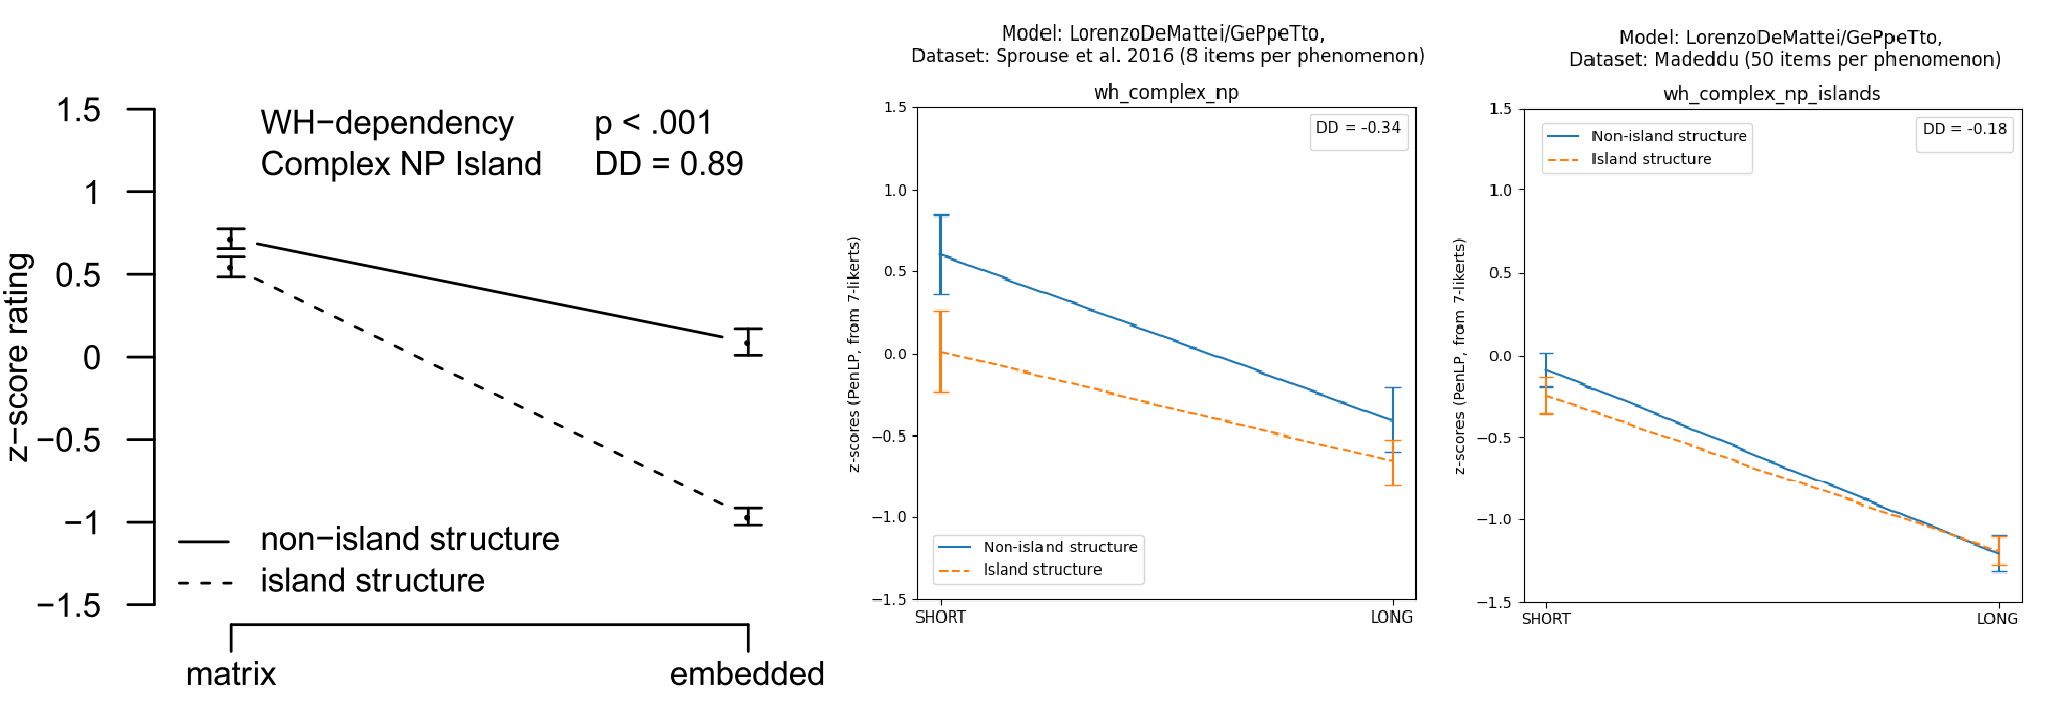
\includegraphics[width=1\textwidth]{images/Chapter1/combined_wh-complex.png} 
	\caption{Comparison of plots for wh-dependencies complex NP islands} 
	\label{fig:wh_complex} % this internally labels the figure for future referencing.
	\medskip
	\small
	The first plot on the left shows the scores on humans subjects published in \citet{sprouse2016experimental} for Italian complex NP islands with wh-dependencies. For each line, the left-most edge represents the score for the short-distance dependency sentence, the right-most the long-distance dependency. The plot in the middle shows the scores from a Gpt-2 model \citep{de2020geppetto} on the same test suite used for the first plot. The plot on the right shows the scores from the same Gpt-2 model but on the expanded test suite developed for the present thesis.
\end{figure}

Doing some variations experiments (see  \autoref{tab:compare1}), we found that by replacing the main clause verbs with "intuire che"/"avere l'intuizione che" ("to sense that" / "to have the intuition that") or "avvertire che"/"avere il sentore che" ("to feel that" / "to have an inkling that") or "percepire che"/"avere la percezione che" ("feel that"/"to have the feeling that"), the island restriction violation seem to have no effect, and the Long-Island sentence becomes more acceptable than the same sentence without the island structure (Long-NonIsland).
 
Indeed, the sentence \textit{Cosa hai avuto l'intuizione che il portavoce avrebbe confermato?} (\textit{`What did you have the intuition that the spokeperson had confirmed?'}), seems acceptable despite extracting from a complex NP construct. 

An hypothesis, whose demonstration we leave for future work, is that this is due to main clause expressions in which the subject has the semantic role of an \textsc{experiencer} rather than an \textsc{agent}, which could be a condition for Complex NP island restrictions to enter into effect or not. 
% "avrebbe ppt" (condizionale passato)
% In fact, it seems that the Gpt-2 model correctly captures the fact that with these constructs the long nonisland sentences become acceptable.

\begin{table} \scriptsize 
	\begin{center}
		\begin{tabular}
			{p{0.3\linewidth} p{0.08\linewidth} p{0.3\linewidth} p{0.08\linewidth} p{0.08\linewidth}|} \\
			\multicolumn{2}{c}{\textbf{\textsc{Long-NonIsland}}} & \multicolumn{2}{c}{\textbf{\textsc{Long-Island}}}  &   \\
			\textbf{text} & \textbf{PenLP} & \textbf{text} & \textbf{PenLP} &  \textbf{Diff}  \\
			\hline
			\textit{Cosa hai messo in dubbio che il portavoce avrebbe confermato?} & -31.65
			& \textit{Cosa hai messo in dubbio la previsione che il portavoce avrebbe confermato} & -33.21 & 1.56 \\ 
			\textit{Cosa hai intuito che il portavoce avrebbe confermato?} & -32.36 
			& \textit{Cosa hai avuto l'intuizione che il portavoce avrebbe confermato?} & -29.99 & -2.37 \\ 	
			% TODO: use the other verbs too:  "avvertire che"/"avere il sentore che" ,  "percepire che"/"avere la percezione che" 
			\textit{Cosa hai detto che Gianni avrebbe sollevato?} & -33.74 
			& \textit{Cosa hai riferito il fatto che Gianni avrebbe sollevato?} & -36.64 & 2.90 \\ 
			\textit{Cosa hai intuito che Gianni avrebbe sollevato?} & -34.31 
			& \textit{Cosa hai avuto l'intuizione che Gianni avrebbe sollevato?} & -30.52  & -3.79 \\ 
			
			\textit{Cosa hai messo in dubbio che io avrei vinto?} & -26.48 & 
			\textit{Cosa hai messo in dubbio la previsione che io avrei vinto?} & -30.17 & 3.69\\ 				
			\textit{Cosa hai intuito che che io avrei vinto?} & -29.49 & 
			\textit{Cosa hai avuto l'intuizione che io avrei vinto?} & -24.45  & -5.04 \\ 				

		\end{tabular}
		\caption{Comparing acceptability variations among sentences in the complex NP dataset. A positive difference indicates that the Long-NonIsland sentence is more acceptable than the Long-NonIsland one, as expected.}
		\label{tab:compare1}
	\end{center}
\end{table}


\bigskip
% TODO: insert plot of variations
With other variations experiments, we found that replacing the main clause verb with "sapeva che"/"conosceva che" ("he knew that", see examples in table ..TODO), increases the acceptability of the long-non island sentences; on the other hand, this variation results in a lower acceptability to the short island sentence, compared to the scores from human subjects, and by this way the non-island and island line end up being almost parallel, with the DD score close to zero (which indicates an almost absent island effect).
\\ 
%TODO: add table and plots of senteces with  "sapeva che"/"conosceva che" 

% todo: show tables with examples "sapeva che" % todo: numbered examples like formulas
% todo: show the plots for "intuizione che", "sapeva che" (two subfigures, each numbered/lettered to be referenced)

% examples of complex np items before and after the "avuto l'intuizione che" variation: ..
% show the plots for the items using this construct ("avuto l'intuizione che" ), it seems strange scores are given
% (the island line is higher than the non island one, but they are all acceptable sentence and there is no island restriction anymore)

% still the problem overall in the orginal plots seems an overly low score for the long non island sentences
% that is, is the long distance depencency that receives a too loo score .. (lenght effect?)
% while the structure effect ..
% albeit it's correct, like humans scores, that the long non island has less acceptability than the short island
% then how is the long distance dependency (lenght effect) scored for the other island phenomena?
% the difference with the sentences for the other phenomena seem to be that they have a simpler main clause, like "cosa pensi che" (present) + "abbia ppt"  (congiuntivo passato), while for the complex np, is "cosa hai smentito/annunciato/raccontato/sostenuto che" (passato prossimo) + "avrebbe ppt" (condizionale passato)
% a comparison example could be to turn the other 3 island phenomena items into passato prossimo for the main clause
% but was this discrepancy also in Sprouse data, and is this the reason for their plots differences too? (so the gpt2 model just accentuates this drop in acceptability?)

% for future work: automatic generation of examples from templates, like in BLiMP, to control and test more easily for more factors (es. verbs moods and tenses)
% to test for frequency effect: use some rare verb moods/tenses?

% also find an explanation for the other misclassified long non island sentences that use other constructus (with proper agent/patient semantic roles)

% table..

% Mostra una non robustezza del modello nell’apprendimento di strutture sintattiche / or of this use for scoring minimal pairs, non generalizzazione sintattica, in quanto basta una variazione lessicale, anche tra ..parole frequenti, ..per ..alterare ..quale tra due frasi coppie minime sia piu o meno accettabile.
% However, we refer back to section .., about the interpretation/meaning of the Gpt-2 loss ..output/score.


% TODO: table with example items with different constructs, and their scores
% TODO: plots of the whole test suite for this phenomenon with the same variation for all items (using a different verb)



\subsubsection{Whether islands}

From \autoref{fig:wh_whether} for whether islands with wh-dependencies, we can see that the Gtp-2 model, with the PenLP sentence acceptability estimate, compared with the results from humans gives higher scores for all sentence types. This difference is more pronounced in the scores performed by Gpt on the original test suite from \citet{sprouse2016experimental} (middle image). 

The slope of the lines (both for island and non-island sentence structures) is however quite similar to the human scores. \\


\begin{figure}[H]
	\centering
	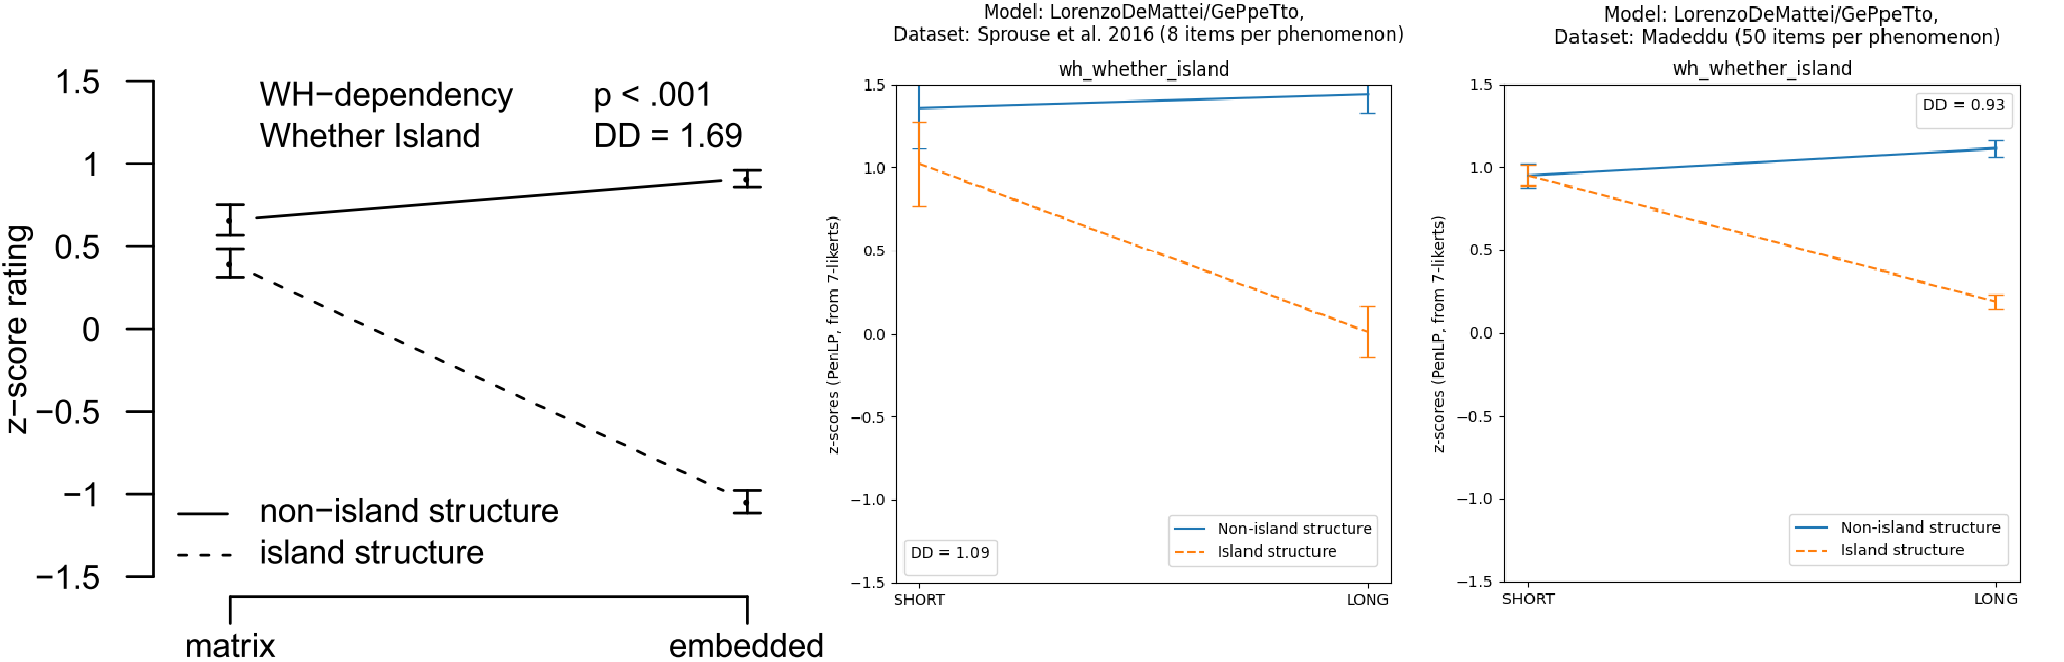
\includegraphics[width=1\textwidth]{images/Chapter1/combined_wh-whether.png} % width= 0.8\textwidth
	\caption{Comparison of wh-dependency whether islands} 
	\label{fig:wh_whether} % this internally labels the figure for future referencing.
\end{figure}

..

% TODO: table showing accuracy scores for the 4 sentences of an item; comparison on variations across multiple items

Experimenting with other sentence variations for whether islands, we found that a variation that aligns the plots more to those from the humans' scores, is replacing the personal pronouns (like "io") with proper nouns (like "Gianni") or common nouns (like “il parlamentare”, or “lo studente”)  like in this example: 

\begin{example}	\textsc{Whether islands, Long-Island sentence type}
	\renewcommand{\labelenumi}{\alph{enumi}.}
	\begin{enumerate}
		\item 
		Cosa ti domandi se io abbia riscosso?
		\item 
		Cosa ti domandi se Gianni abbia riscosso?
		\item 
		Cosa ti domandi se il parlamentare abbia riscosso?
	\end{enumerate}
	\label{variation_2}
\end{example}

% This might be the reason for the discrepancies in some of the 4 phenomena: some make more use of ..nomen agentis, while others rely more on personal pronuns. Try this replacement this in all 4 test sets.
%TODO: put scores values and/or to quantify the effect of these variations.

TODO: test sentence variations using less common verb tenses and moods (but consistently across an item or even all items of a suite)
% Not much difference seems to derive by using less common (..) verbs
% (examples in which both sentences in a pair also specify the direct object, see how this affects the score? Like long nonisland vs long island ..)


\subsubsection{Subject islands}

\begin{figure}[H]
	\centering
	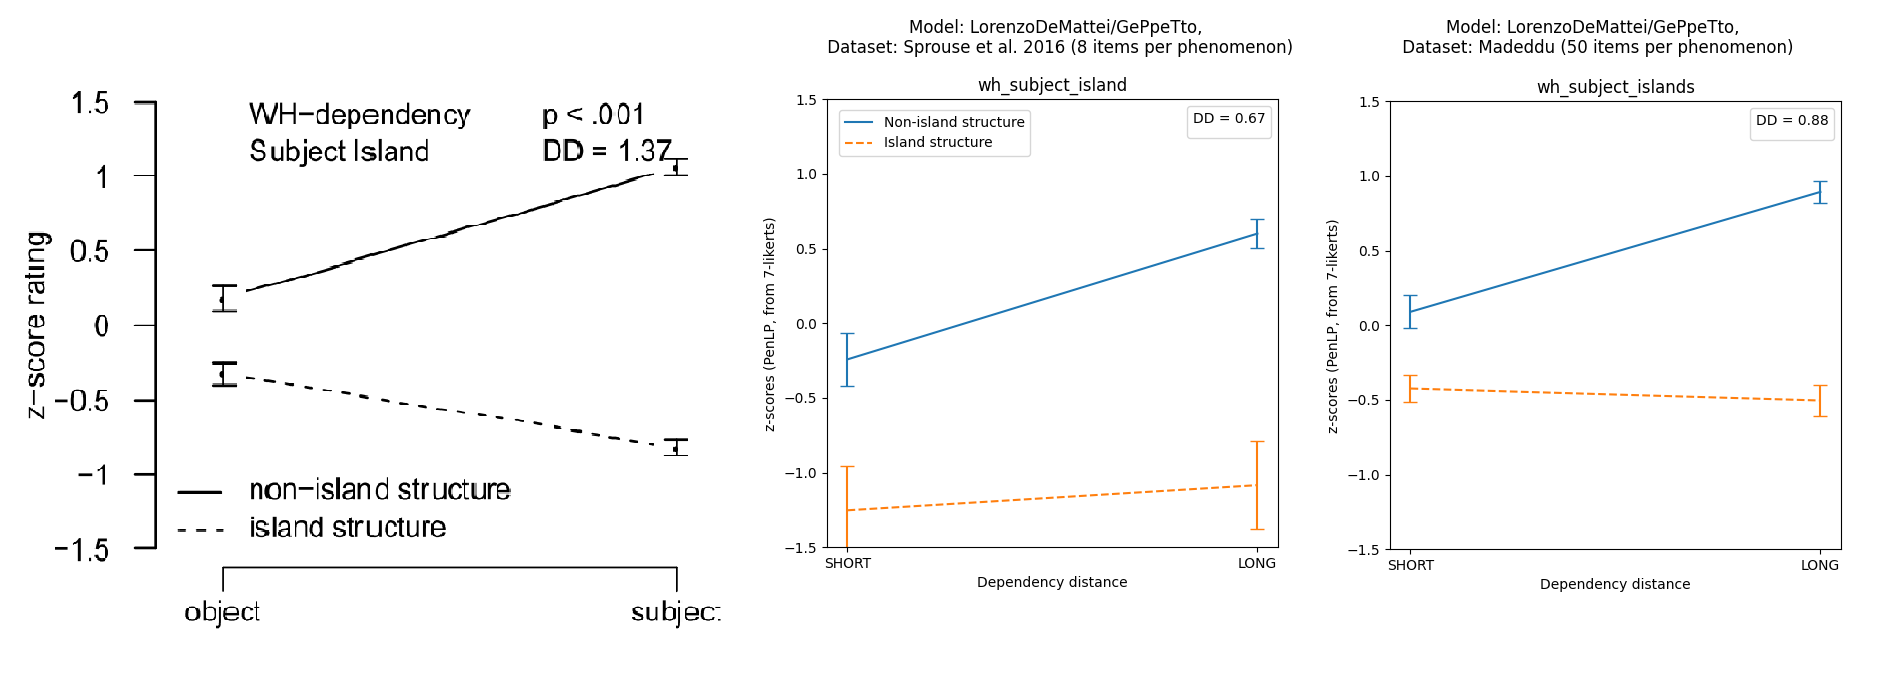
\includegraphics[width=1\textwidth]{images/Chapter1/combined_wh-subject.png} 
	\caption{Comparison of wh-dependencies subject islands} 
	\label{fig:wh_subject} % this internally labels the figure for future referencing.
\end{figure}

In \autoref{fig:wh_subject}, the middle image of Gpt scores on Sprouse data shows significantly lower scores (compared to the human scores on the left image) for the sentences with an island structure (dotted line). % check the sorting of sentences to see why). 
However, on the right image (Gpt scores on our test suite) they are similar to the human scores. \\

For the non island line, the Short-NonIsland is scored lower then on human subject by Gpt for both testsuites. The Long-NonIsland scores instead are similar  (around 1.0). % but lower on sprouse data. \\
The slope of the lines on the right image is similar to the one for the human scores (left image). %  oneon the model scores, both for sprouse and new data, but steeper compared to acceptability results on human subjects.


\subsubsection{Adjunct islands}

\begin{figure}[H]
	\centering
	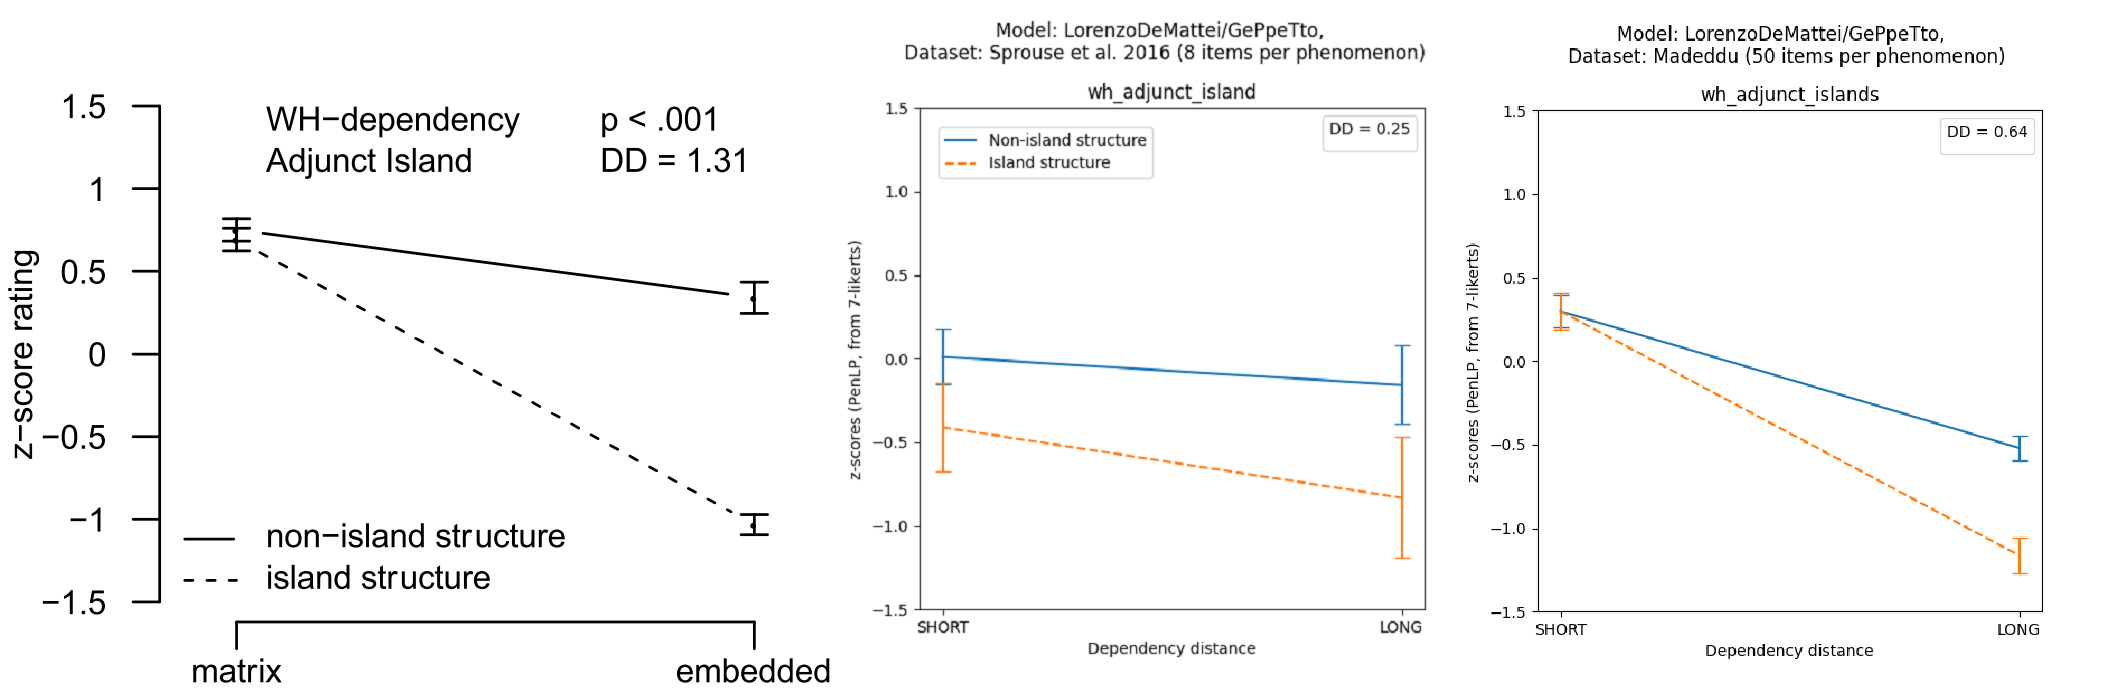
\includegraphics[width=1\textwidth]{images/Chapter1/combined_wh-adjunct.png} 
	\caption{Comparison of wh-dependencies adjunct islands} 
	\label{fig:wh_adjunct} % this internally labels the figure for future referencing.
\end{figure}


In \autoref{fig:wh_adjunct} the slope of both lines on the new test suite (right image) is similar to the human scores (left image), althoughg with a lower average acceptability for the Long-NonIsland sentences, which results in a downward steeper line. 

Note that in the test suite we developed for this thesis, the Long-Island sentences for adjunct islands have a form that might make them more easily identifiable has unacceptable than the ones in the Sprouse test suite: compare \textit{Che cosa Gianni è partito per Parigi dopo aver fatto?} (new dataset) with \textit{Cosa ti irriti se dimentico in ufficio?}. The ending of the first sentence might be less frequent and result in a lower acceptability score.
% in the sprouse data, at the end there is a preprositional ..phrase like “in ufficio”.


\subsubsection{Overall observations across all four island phenomena}

The Gpt-2 scores on the original Sprouse et al. test suite (middle image) have wider standard error bars, which are considerably smaller for the new test suite developed for the present thesis (right image).\footnote{This might be due to the fact that the number of items between the two test suites increases from 8 to 50.}


While on human ratings the unacceptable sentences (Long-NonIslands) receive all on average a z-score of about -1, there is more variability in the scores given by the Gpt model, in particular for whether islands sentences (\autoref{fig:wh_whether}), which receive much higher acceptability rating on average (betwenn 0 and 0.5 the Sprouse test suite and ours).
..

% TODO: remaining tables with accuracy scores, comparison with BLiMP extraction islands scores; compare btw models, scoring measures, and datasets (BLiMP, Sprouse, Madeddu)

% todo: all the plots in the appendix (BERT, LP/PenLP, logistic LP/PenLP, .. ) and brief comments 
% (like limitations of BERT acceptability estimates)

% Italian models:
% "LorenzoDeMattei/GePpeTto"
% "dbmdz/bert-base-italian-xxl-cased": ModelTypes.BERT,
% "idb-ita/gilberto-uncased-from-camembert"

% testsuites/datasources:
% Sprouse et al.
% Madeddu

% scoring measures:
% LP/PenLP (softmax-based)
% % LP/PenLP (logistic-based)


\subsection{Discussion on plots from BERT, the logistic function, and PenLP}

% BERT-like models, LP/PenLP scores also based on logistic function scores
% (comment also on the accuracy scores from other models?)

In \autoref{fig:bert_penlp_l_sprouse} we see the plots of the scores from the BERT model, with the PenLP-L sentence acceptability estimate (using the logistic function rather than the softmax, as described in \autoref{sec:softmax}). Interestingly, it seems that this combination of BERT with the logistic function makes a clear separation between unacceptable sentences (the Long-NonIsland type) and acceptable sentence types, with minimal, if any, difference in score between acceptable sentences.

\begin{figure}[H]
	\centering
	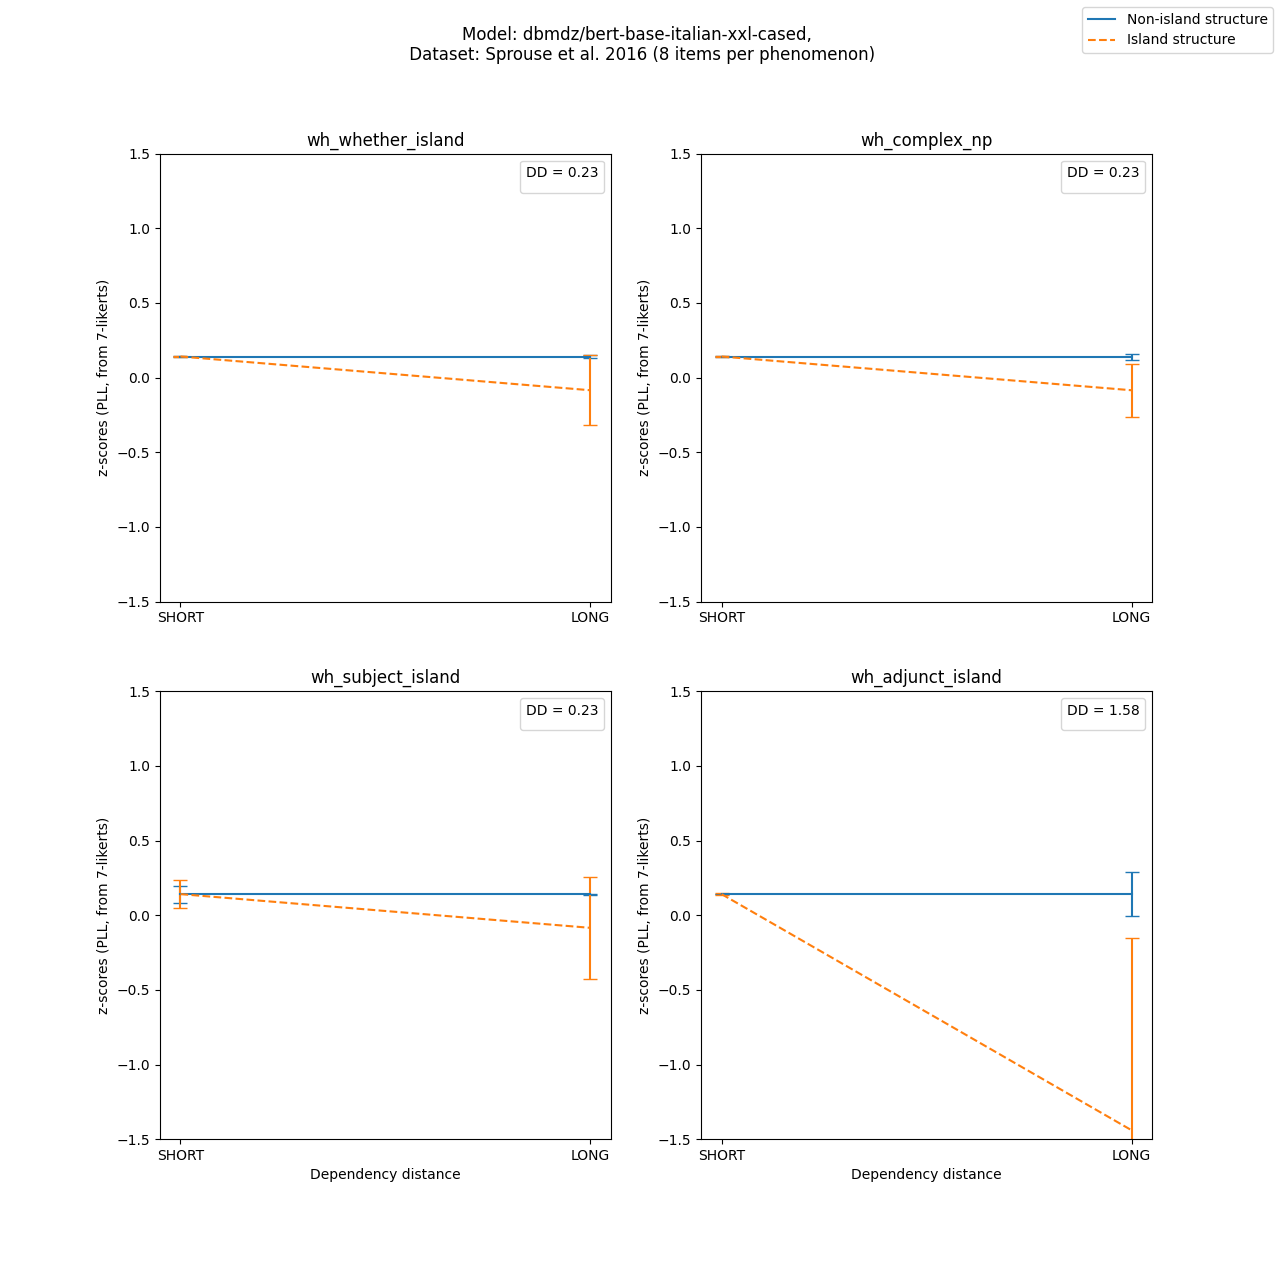
\includegraphics[width=1\textwidth]{images/AppendixA/Sprouse_wh_dbmdz_bert-base-italian-xxl-cased_PLL-zscores-likert-2022-07-11.png} 
	\caption{Plots from BERT with the PenLP-L sentence acceptability approximation}
	\label{fig:bert_penlp_l_sprouse}
\end{figure}

If we compare these plots with the accuracy scores in \autoref{tab:accuracy_it_data} from this model (BERT, logistic function, PenLP) , we see that they are among the best with an average accuracy of 80.7\%; however, looking at the scores for each phenomenon, the scores are high only in about half the cases, and quite low for the rest: Long-NonIsland sentences of all four island phenomena are scored with 58\%, 64\%, 74\%, 58\% accuracy, and the Short-NonIsland of subject islands with 28\% accuracy.

%TODO: check if this is also a skewing effect of the normalization (from the likert scale and the z-scores) and the presence of much negative large values for the unacceptable sentences: in this case the normalization would ..squeeze together the score for the acceptable sentences, if they have a smaller magnitude.

% With the , the use of the logistic function scores as a basis for LP/PenLP instead results in much ..worse plots (  ). Whether, complex and subject islands get almost identical plots, due to the ..skewing/normalization effect of the discretization and the zscores, because the adjunct islands have much higher magnitude negative values (low acceptability) for the unacceptable sentence (long island.) (? so it seems that with BERT and logistic function scores emerge more clearly a distinction between acceptable and unacceptable sentences, without much differenciation within these two groups).

\subsection{Discussion on plots from GilBERTo}

Overall, for GilBERTo, the plots are significantly different from those on human ratings. (..)

\begin{figure}[H]
	\centering
	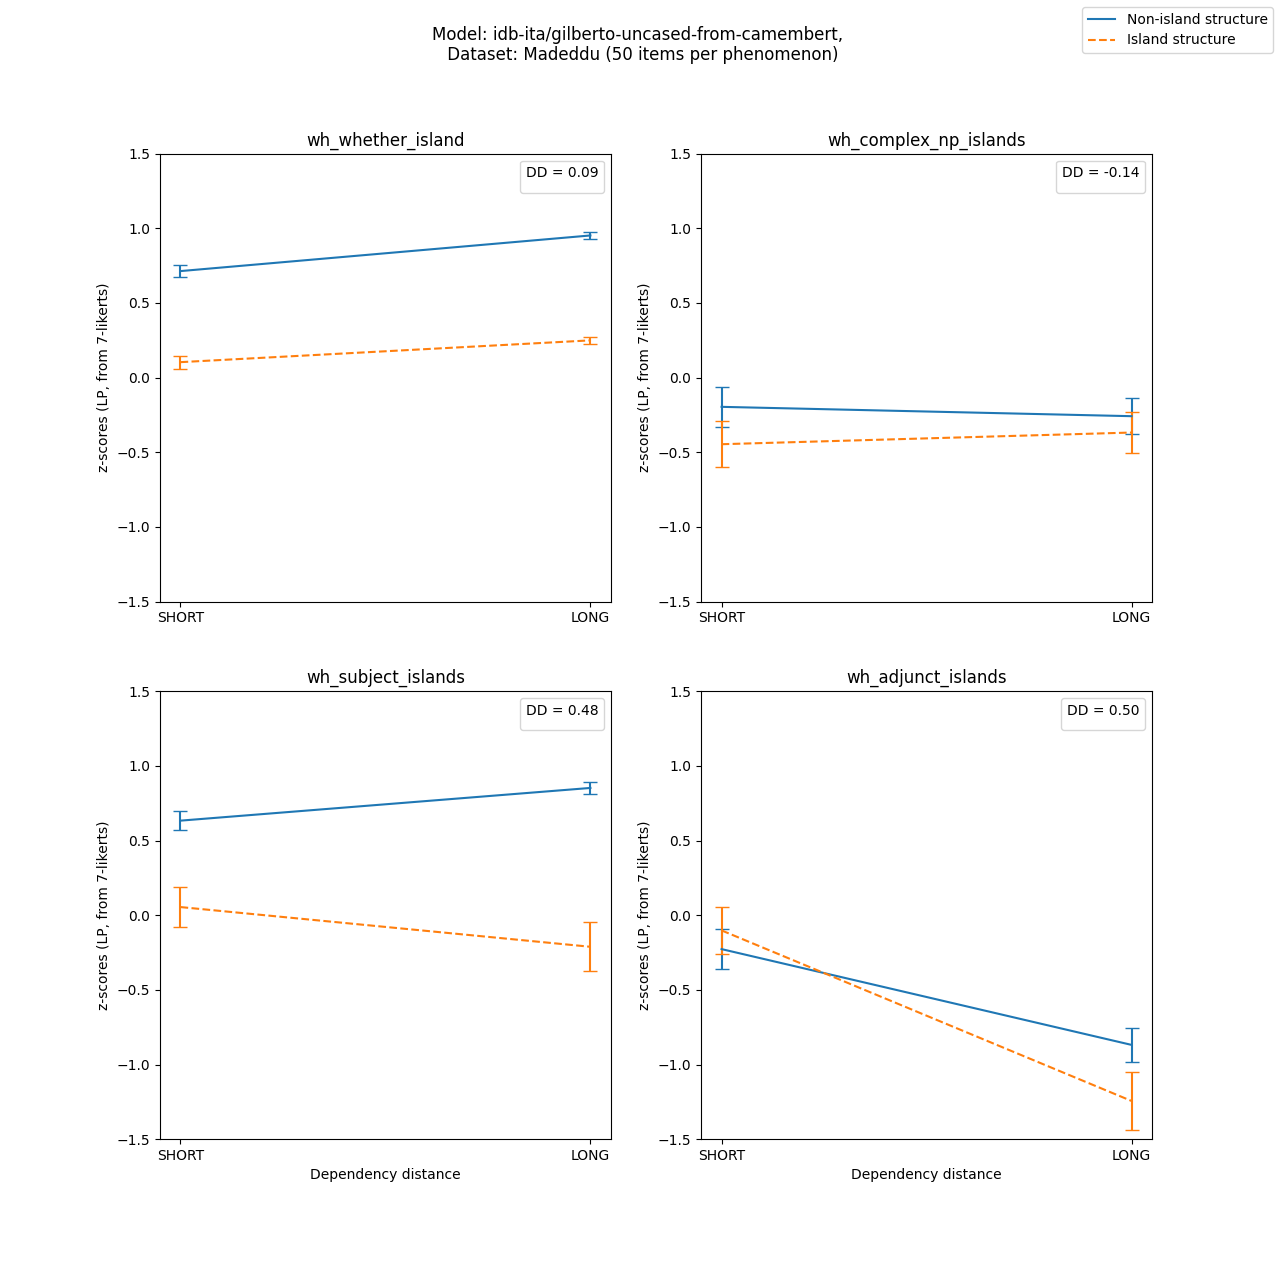
\includegraphics[width=1\textwidth]{images/AppendixA/Madeddu_wh_idb-ita_gilberto-uncased-from-camembert_LP-zscores-likert-2022-07-11.png} 
	\caption{Plots from GilBERTo with the LP sentence acceptability approximation}
	\label{fig:gilberto_lp_madeddu}
\end{figure}


\section{Draft notes on the results}
\subsection{Observation on plots for other models}


The plots for Geppetto and PenLp are the most similar to the plots on human ratings. However, with the LP measure, the plots differ significantly.

The plots for BERT with PenLP on the Sprouse data are similar to the results on humans from \citet{sprouse2016experimental}, %..with some ..differences..


In the plots from the GilBERTo scores, we see that for complex NP and subject islands, the sentences with the island structure receive a higher acceptability than the non island ones (this is no longer the case when removing the penalty for sentence lenght, using the LP sentence acceptability measure). With the PenLP sentence acceptability approximation, the lines tend to have similar slopes, close to being parallel (indicating a lack of, or small, island effect). 

%
%Plots on the Madeddu dataset developed for the present thesis:
%
%BERT, softmax, PenLP and LP
%..
%for adjunct islands, LP seem to work best (without penalizing for sentence lenght).
%Using the logistic function scores, again we see the ..binary differentiation btween unacceptable (long non island) and acceptable (the other 3 types) sentences. However here the plots are more ..flattened, with the scores being very close to the same values.

We refer to the Appendix for the plots for the other models.

\subsection{What seems to affect the models acceptability scores}


\subsubsection{Adjunct islands}

Guardando le short-nonislands, sembra anche qui preponderante il fatto di usare nomi propri di persona (che ha uno score di accettabilità minore) e usare invece di nomi comuni animati/di mestieri/.. (che aumenta l’accettabilità). Ma questo non sembra influenzare il DD score finale % (..evidentemente i vari fattori si bilanciano).


\subsection{Discarded observations on differences between the plots}

\subsubsection{Other notes on  Complex np islands,  what seems to affect the models acceptability scores}
In \autoref{fig:wh_complex} we see that the non-island line (the line connecting the two acceptability scores for short and long distance dependency sentences without an island structure) is significantly lower in new data (todo: see constructs that increase the score of both long and short)

The (gpt) model seem not to make much difference in ..acceptability btw “regular” subordinates and complex noun phrases ..

-- also the short island point is significantly lower

All the 50 + 8 items of the two test suites (the ones from Sprouse et al and the ones developed for the present thesis), when altered to use the following construct for the complex NP "avuto l'intuizione che" (had the intuition that), are scored by the model as if there is no island restriction violation anymore. 

il verbo “intuire” diminuisce ..l’accuratezza del giudizio di accettabilità
in particolare diminuzione della accettabilità delle frasi long nonisland (con long distance wh dependency e struttura non island), che ricevono accettabilità minore di quelle con struttura island:
Esempio analisi variazioni con verbo “intuire” complex np, ..

the verb form “sapeva” (imperfect), compared to ..present perfect forms (“ha osservato/affermato/..”) seems to get better DD score in complex np islands (and also in another phenomenon ..).

\subsubsection{Whether islands}
NB: note that according to human scores, for this type of whether island sentences, the "correct" scoring is to have an increase in acceptability going from short to long non island sentences.
Maybe comparing the scores between acceptable sentences (in this case short and long non islands), expecting it to match humans acceptability judgements .. is beside the present ..research question.
In any case, we noted a reverse in the acceptability difference between this two types of sentences (short and long non islands) when changing the subject of the subordinate sentence from a personal pronoun ("io", 1st pers sg), to a proper noun (i.e. "Gianni"), to a common noun (i.e. "il parlamentare").

%-- significant variation in acceptability diff between short non island and long non island, when replacing: the personal pronouns io/lei, with a proper noun like "Gianni", or even more with a noun like "il parlamentare" (the congressman). In this latter case, significant improvement toward the expected acceptability rate (only 10 out of 50 are .."missclassified"). With the proper noun "Gianni", 18 are missclassified. With the personal pronoun 29 out of 50 are missclassified.
%Try replacing with .. another proper noun, more common like ..
%
%
%(tables and examples of these variations to put on the thesis/report?)
%
%(possible explanation: personal pronouns and proper nouns might be less common in the type/genre of corpora these models were trained on, like wikipedia).
%Observations: the direct objects in the examples are all relatively common words..\footnote{\citet{wei2021frequency} found significant frequency effects (but for agreement .. tests, which are much easier to isolate), for items that occurr rarely in the training corpus (..less then ..10-100 times). But to notice this effect they had to purposly tweak the training corpus. Replicating this for a preexisting corpus (using very rare vocabulary ..) is much more complex and out of the scope of the present study.}
%try with rarer ones.
%..
%-- both on sprouse and new data, gpt "incorrectly" increases the accceptability from short to long non island (check constructs that instead decrease the acceptability?)


\section{BLiMP English dataset}
..
\subsection{English models details}
..

\section{Token surprisal analysis}

(TODO)
%We found the most informative analysis (rather than the factorial test design) was looking at the token surprisals for the Bert-like models (do it also on the Gpt2 logits?).
%..
%(even more informative, or complementary, would be to look at the activations in the model layers)
%
%
%
%"The ratio of token-level PPPLs between unacceptable and
%acceptable sentences overall increases with performance, separating the two sentence sets" \citep{salazar2020masked}
% plot token surprisal on Blimp sentences, compare spikes of minimal pairs differing for just one word


\section{Follow up experiments and future work}

(..)
% finetune the models for acceptability? (already existin italian models for this, like from Trotta et al. 2021?)
% finetuning is very fast anyway 
% (fine tune also for english the Bostrom models?)

% (also to the plot on acceptability score by sentence lenght?)

% what about a follow up analysis on the thesis, based on the results? like manipulating data to check the effect of somee factors, ..


%Analizzare le attivazioni nei vari livelli del modello ..
%Fare un training .”a strati”, in cui in ciascuno strato c’è il target dell’apprendimento di un livello di base della lingua (morfologia, sintassi, semantica, ampiezza del vocabolario, ..), con strati successivi che aumentano la complessità della conoscenza che il modello ha del linguaggio.
%
%
%Confronto percentuali accuratezza (short/long non island, short island) con quelle in BLiMP
%(and other works with extraction islands evaluations?)

\chapter{Conclusions}
..

\chapter{Note sections to remove}
\section{misc ideas with notes}

..
(misc ideas with notes)
using multiple POS taggers and semantic role taggers etc.
one, the default, for most common (..more prototypical) sentences/structures
the other ones, used in ..garden path scenarios, when multiple indicators show that some POS tags or semantic role or other category might be wrong.
the second set of taggers should do a ..full parsing analysis.. combining and ranking different parsing hypotheses)


(on perplexity: the target of "low perplexity" in a language model, should not be in the ..words themselves, because language has informative/comunicative goals that are to introduce new, less predictable, information; it should be at other levels, like that of correctedness/acceptability; target of low perplexity of POS tags, semantic role tags, etc.) \\
\citet{von2018pos} use perplexity on POS tags as a measure of syntactic complexity;
"working on POS sequences avoids having to deal with data sparsity issues." \citep{von2018pos}

what about using perplexity on POS tags as a measure/estimation of syntactic well formedness?
": Lawrence et al. (2000) train RNNs to do
acceptability classification over sequences of POS
tags corresponding to example sentences from a
syntax textbook."

discriminate btw complex/rare vs unacceptable? a threshold (linearly separable) on perplexity? Or multiple dimensions, non linearly, should be used?
(but if there is a wrong/mispelled word.. the pos tagger might misclassify it)
(distinguishing ..sentence unacceptability by linguistic level: morphological mistakes/typos, ..word order errors, ..)
(also: perplexity uses a markov model of language? no, but multiplication the perplexity of each word to obtain the perplexity of the whole sequence.. a "less linear" formula might be needed..)
(montemagni et al paper on profileU on linguistic profiling? use for sentence acceptability estimates? use for ..style detection/automated analysis ..


\section{Misc notes with refs}


First work with targeted syntactic tests on modern language models (RNNs or transformers) is \citet{linzen2016assessing}, while first use of psycholinguistic tests for modern LM is from \citet{futrell2018rnns}.

“NATURAL LANGUAGE DOES NOT MAXIMIZE PROBABILITY” 
“Why is human-written text not the most probable text? We conjecture that this is an intrinsic property of human language. Language models that assign probabilities one word at a time without a global model of the text will have trouble capturing this effect. Grice’s Maxims of Communication (Grice, 1975) show that people optimize against stating the obvious. Thus, making every word as predictable as possible will be disfavored. This makes solving the problem simply by training larger models or improving neural architectures using standard per-word learning objectives unlikely: such models are forced to favor the lowest common denominator, rather than informative language.” 
\citep{holtzman2019curious}

Repeated exposure to a type of island construct will increase its perceived acceptability 
\citep{chaves2014subject}



"Auxiliary training objectives Adding auxiliary unsupervised training objectives is an alternative form of semi-supervised learning. Early work by Collobert and Weston [10] used a wide variety of auxiliary NLP tasks such as POS tagging, chunking, named entity recognition, and language modeling to improve semantic role labeling. More recently, Rei [50] added an auxiliary language modeling objective to their target task objective and demonstrated performance gains on sequence labeling tasks. Our experiments also use an auxiliary objective, but as we show, unsupervised pre-training already learns several linguistic aspects relevant to target tasks." (Radford Gpt)

survey on alternative training tasks etc.: paper "a primer on BERTology"

"QUALITATIVE ANALYSIS" (REASONING ABOUT ENTAILMENT WITH NEURAL ATTENTION, Tim Rocktaschel et al. 2016)

"Efficiency considerations are important when building language models that use
such large sets of n-grams. Rather than store each word as a string, it is generally
represented in memory as a 64-bit hash number, with the words themselves stored
on disk. Probabilities are generally quantized using only 4-8 bits (instead of 8-byte floats), and n-grams are stored in reverse tries." (Jurafsky 2021 3rd ef ch.3)

"the standard information theory textbook Cover and Thomas (1991). "

"It uses the output of a character-level
Convolutional Neural Network (CNN) as input to
the LSTM. This model has the best published perplexity for English text." \citep{wilcox2018rnn}

\section{Notes and refs on incorporating explicit semantic info}

% "Syntax in LMs: There have been several proposals over the years to incorporate explicit syntax into LMs" ", in practice it can still be beneficial to inject syntax into the model. This can be done by combining it with a supervised parser (Dyer et al., 2016) or other multi-task learning objectives (Enguehard et al., 2017)" \citep{marvin2018targeted}

% "Multi-task training with a syntactic objective (CCG supertagging) mitigated this drop in performance for some but not all of the dependencies we tested. We conjecture that the benefits of the inductive bias conferred by multi-task learning will be amplified when the amount of training data is limited"  \citep{marvin2018targeted}
% (that is, incorporating linguitic signals could be effective in lowering the amount of training data needed)

% "Second, we find a larger effect of model inductive bias than training data size on SG score, a result that accords with van Schijndel et al. (2019). Models afforded explicit structural supervision during training outperform other models: One structurally supervised model is able to achieve the same SG scores as a purely sequence-based model trained on ∼100 times the number of tokens. Furthermore, several Transformer models achieve the same SG score as a Transformer trained on ∼200 times the amount of data. " \citep{hu2020systematic}

% Alternative training tasks:
% "Task reformulation: Language model is usually pre-trained with a Masked Language Modeling (MLM) objective, which is motivated by Cloze task in (Taylor, 1953). There have been several works reformulating few-shot learning tasks as cloze questions to reuse pre-trained LM such as LM prompt (Jiang et al., 2020), PET (Radford et al., 2019; Schick \& Schutze, 2020a), and recent ¨ LM-BFF (Gao et al., 2020). It shows a pre-trained LM can achieve non-trivial performance with few annotated samples. There are also some other works transforming NLP tasks as generative QA tasks (Puri \& Catanzaro, 2019)." but low performance on CoLA (possible beacuse of "different data distribution"): "The only exception is the CoLA (the linguistic acceptability task). It is might due to that MLM pre-trainng and entailment training did not see this type of data distribution before"

% enriched training data (with supervised tasks): "Intermediate training: The work by (Phang et al., 2018) shows that supplementing pre-trained LMs with further training on data-rich supervised tasks can obtain additional performance improvements on the GLUE benchmark."

% Freezing / Frozen Layers:
% "The results align with Lee et al. (2019), who discuss the performance degradation of BERT-based models depending upon the number of frozen layers." (Cherniavskii et al. 2022)

% \nocite{wei2021frequency, hu2020systematic, lau2020furiously, bostrom2020byte, futrell-etal-2019-neural}
